\documentclass[a4paper,12pt]{report}      % Specifies the document class

% Add packages here
\usepackage{enumerate} % for lists
\usepackage{natbib}    % for bibtex
\usepackage{graphicx}  % for images
\usepackage{fixltx2e}  % for subscript
\usepackage{seqsplit}  % for splitting URIs
\usepackage{arabtex}   % for acks
\usepackage{utf8}      % for arabic
\usepackage{atbegshi}  % to skip first page

% The preamble begins here.

% Custom macros

% Title
\title{Master's Thesis:\endgraf An Investigation into the application of Content-Centric Networking within Challenged Network Environments using CCNx}
\author{Tarek Elshaarani - tarek@tekbase.org } 
\date{\parbox{\linewidth}{\centering
  \bigskip
  \today\endgraf
  \vspace*{7cm}
  Supervisors: \endgraf
  \hspace*{1cm} Frederik Hermans   - frederik.hermans@it.uu.se \endgraf
  \hspace*{1cm} Ferdrik Bjurefors  - fredrik.bjurefors@it.uu.se \endgraf
  \bigskip
  Reviewer: \endgraf
  \hspace*{1cm} Christian Rohner   - christian.rohner@it.uu.se \endgraf
  \bigskip\bigskip
  Department of Information Technology\endgraf
  Uppsala Universitet}}

% Document
\begin{document}             % End of preamble and beginning of text.
\maketitle

%% TODO: Fix formatting - numbers according to https://www.it.uu.se/edu/exjobb/master/rapporten

% Blank page to please the formatting gods.

\pagebreak
\chapter*{Abstract}

Information Centric Network (ICN) architectures offer a viable alternative to conventional TCP/IP designs to cope with the disruptive nature of Challenged Network environments. They aim to address the challenges of unreliable connectivity and location transparency to present a delay- and disruption-tolerant solution. This thesis introduces Named Data Networking (NDN), a prominent ICN architecture, that uses a publish/subscribe-driven model and relies on two main message units for communication, called Interests and Content Objects. Instead of a host-based model for data retrieval, an addressing scheme based on named data is utilized. The naming of data allows for retrieval of data from the network without the knowledge of individual hosts. 

This thesis studies CCNx as an implementation of a Content-Centric Networking protocol that inherits key characteristics from NDN. We study the behavior of of CCNx using the Haggle testbed to simulate a simple disruptive network environment. We then develop a delay/disruption-tolerant framework based on CCNx and build an implementation of the game Tic-Tac-Toe using that framework. The framework design is presented with an analysis into various alternatives that were considered. A more complex five-node experiment with link disruption is performed using the framework to evaluate CCNx in a real world scenario. We conclude that CCNx is a good contender for use in Challenged Networks.



% Another blank page because you can never waste enough paper.

\pagebreak
\chapter*{Acknowledgements}

%
% TODO: Remember to add Acknowledgements.
% 
%
% In memory of 25 January 2011, 30 June 2012, and other victorious days to come.
%\setcode{utf8}
%\< عيش ؛ حرية ؛ عدالة اجتماعية >
%

\tableofcontents

% Another blank page to force text to start on an odd number (because even numbers are evil).


\pagebreak
\chapter{Introduction}
A boom in user-generated content along with the widespread use of social networks has created a significant increase in the amount of data generated on a daily basis. A major contributor to this increase is the ubiquity of mobile devices that allow users to generate and consume data without being restricted to location. Despite the advances in wireless communications that allow larger coverage areas and higher transmission rates, current networks fall short in situations where there is no connectivity due to geographical limitations or when there are disruptions that affect the infrastructure. Such situations present two main challenges with regards to data distribution: 1) \emph{Unreliable connectivity} 2) \emph{Location transparency}. There is a continuous effort to improve upon both factors to enhance user experience. This thesis investigates Content-Centric Networking (CCN) as one such paradigm that
attempts to overcome these challenges.

% {TCP/IP shortcomings with handling re-transmissions, and high latency/long distances}
\paragraph{Unreliable Connectivity}
The conventional method of data distribution involves end-to-end connection between nodes on a network to query, publish, and retrieve information. Existing communication protocols offer unsatisfactory performance in situations where connectivity is unreliable. TCP/IP is known to perform poorly in such environments, especially because end-to-end paths between communicating nodes are often unreliable resulting in continuous interruptions\cite{tcpbreak}. 
While TCP/IP has evolved to accommodate different types of networks and suit a variety of environments, it still is not suited for some situations when used over high latency, unreliable, or dynamic networks. This is mainly due to the basic requirement to have an end-to-end connection between hosts for data to be exchanged.

% {Location Transparency}
\paragraph{Location transparency}
Another shortcoming with conventional network architectures is in situations where node location is dynamic due to mobility. If the node holding particular data is not accessible on the network at a particular instance, the information is subsequently unavailable due to the basic requirement of having stable end-to-end connectivity. Furthermore, if the node reconnects to the network from a different location, the data cannot be retrieved from the location it was previously known to be found. The dynamic nature of the nodes makes it unfeasible to use conventional indexing methods that map data to specific locations from which it can be retrieved.

\section{Challenged Networks}  

To address the issues of both intermittent connectivity and location transparency, experimental network
architectures offer different approaches that do not rely on reliable end-to-end connectivity between
nodes or precise knowledge of their location. These alternative architectures are particularly relevant to
one group of networks, henceforth referred to as Challenged Networks. This family of networks
provide a set of unconventional architectures that attempt to address problems that are not offered by
other widely deployed network architectures, namely TCP/IP-based ones. They operate in conditions
where there is a low power requirement, sparse connectivity, frequent mobility, and more importantly,
unpredictable link disruptions. This is particularly true for wireless networks where connectivity can be
intermittent due to power or coverage limitations, interference resulting in re-high transmission rates,
and other mitigating factors. The nature of intermittent connectivity may vary from milliseconds to
hours during often with only small windows of opportunity for data to be exchanged\cite{DTNarch}. 

The characteristics lead to the basic issue that concerns such networks, which is the the lack of
continuous end-to-end communication between nodes. A generally accepted approach applied to
address this drawback is a technique commonly referred to as “store-and-forward”. This in-network caching solution takes advantage of using resources of reachable nodes on the network as intermediaries to store data until it can be routed to the destination.

While they follow those general guidelines, there are several types of Challenged Networks that
address various issues slightly differently than the others and each are a topic of research on their own.
A number of the most prominent are introduced briefly below.

\begin{description}
\item[Delay Tolerant Networks:] Mainly concerned with being resilient to communication delays, high
latency, or round trip times. One application of this network would be in inter-planetary
communication\cite{DTNarch}\cite{rfc4838}. 

\item[Disruption Tolerant Networks:] These are similar to Delay Tolerant Networks, and commonly grouped
with them, but are more related to prevention and recovery from link degradation and disruption. The
nodes on the network must be able to both reconnect from link failures as well as recover from
potential data loss or inconsistency if transfer is interrupted. This may be applicable to high availability
networks and military use\cite{DTNarch}.

\item[Opportunistic Networks:] Commonly considered a subset of Disruption Tolerant Networks, this type of
network makes no assumptions about reliable underlying infrastructure. They are mainly associated
with ad-hoc wireless mobile networks where there is a high rate of mobility and unpredictable
connectivity or coverage between nodes. Due to the lack of consistent connectivity, most
communication is asynchronous and routed on a hop-by-hop basis using opportunistic routing
techniques. This type of network can be used to disseminate information in cases of natural disasters or
censorship\cite{oppnets}.
\end{description}

\section{Information-Centric Networking}
% {ICNs offer a solutions to both issues}

One proposed paradigm that offers a solution for Challenged Networks is Information-Centric
Networking. In contrast to today's IP-based networks which are mainly concerned with host-based
addressing on the network, Information-Centric Networks (ICNs) use naming schemes to label
information that can be queried and retrieved from the network. In this sense, the data distribution
method is abstracted from the node level to an information level and is independent of its location.
Communication is carried out in terms of requesting and publishing named information where the
replication of data is handled at the network layer regardless of the originating source. This
characteristic makes ICN architectures attractive for use in Challenged Network environments
including applications such as content distribution (CDNs), disruption recovery, and \emph{flash-crowd}
handling.

While a number of different ICN architectures have been proposed, they all rely on three basic
principles. The first is that all data is represented as objects, which are manipulated by publish and
subscribe operations obsoleting the importance of data locality. The second is caching is an inherent
part of the architecture supported by all nodes in the network assisting in both the acquisition and
dissemination of information. The third and final principle is objects, representing data, are intrinsically
secure using cryptographic signatures created by the original publisher, which can be verified
by consumers. On the other hand, there are many more characteristics that differ between architectures.
These include naming and name resolution, routing, caching mechanisms, Error and Flow control,
privacy, network heterogeneity, and performance. Each of these properties is worthy of being a research
area of its own account\cite{hotnets}. Nonetheless, ICNs are claimed to be a scalable and
cost-effective solution that may replace conventional end-to-end point networks and offer more in areas 
where such networks are lackluster such as mobility and disruption tolerance.

% { Introduce projects and NDN in specific }
Some of the prominent ICN-based projects include 4WARD, Sail, Pursuit, Connect, and Comet\cite{bond}. 
One of such ICN projects that currently enjoys growing interest from the research
community is Named Data Networking (NDN). NDN is based on principles of an ICN, yet still builds
upon the strengths of host-centric networks\cite{ndnproj}. 

\subsection{Named Data Networking}
% { NDN overview }
As with other ICN architectures, NDN is publish/subscribe-driven using basic message units called
Interest and Data. Interest messages represent requests for data, or Content Objects. 
Data messages carry Content Objects as responses to Interest messages. 
Each node on the network is considered a router, which has one or more interfaces,
commonly referred to as faces. Each node also has the ability to store data in a
 local repository called a Content Store. The Content Store acts as a cache for Content Objects on nodes 
that do not originally hold the data. Content Objects are referred to by a unique naming scheme consistent throughout the network and are all
signed crytographically. Additionally, each node maintains two tables: 1) a Forwarding Information Base
(FIB) that maps Content Object names to faces that they can be found; mainly used for routing 2) a
Pending Interest Table (PIT) that maps Interests to the face from which that they were received.

A requester or consumer of a data controls the flow of communication and it is their responsibility to
ensure that the required data is received correctly. The requester sends out an Interest message on the
network by its unique name. An intermediate node on the network that receives this packet will look
up the requested object in its local Content Store in an attempt to fulfill that request. If that object is
found, then a Data message containing the Content Object is sent back to the over the same face. In the
case that it is not locally cached, an entry is added to a PIT to record where the Interest message came
from. This also helps limit the number of Interests generated on the network as only one will be
forwarded regardless of how many are received by a single node. The node will then use the FIB to
identify the face to route this Interest. Because FIB entries used for routing
can be prefix based, they allow for flexibility in terms of specifying the destination interfaces on which 
messages are to be forwarded. It is also possible to forward a request to all available faces. 
The Interest is forwarded over those faces until it reaches a node which can satisfy that request. 
That node will then use the PIT to identify which face the request came from and send a Data message
 back containing the Content Object requested. Because message traversal information is not stored, 
the return path of the Data message may not necessarily be identical to the one used by the one taken by the corresponding Interest message.
Any intermediate nodes between that node which responds to the request and the original requester will
store the response in their Content Store and remove the entry for that Interest from their PIT\cite{nnc}. 

% { The case of NDN as a solution to Challenged Networks }
Interests can be sent using multicast or broadcast mechanisms to allow for a greater search
space. A Data packet is only sent as a response to a corresponding Interest and a node will only respond
with one Data packet on each face for as many Interests it receives. These properties, along with
Content Store caching, provide means that allow data to be sent returned to the requester efficiently
from a nearby node, with resilience to mobility and link disruption.

While one aim of the NDN project is to build a foundation for the next generation of an Internet-
capable architecture, it is also particularly interesting when applied to Challenged Networks. While it
would theoretically provide a good platform due to the nature of the architecture, it is important to test
and validate these claims in order to identify potential issues or drawbacks and how they can be
addressed\cite{ndnproj}.

\pagebreak
\chapter{Problem Definition and Thesis Contributions}

%{ What this thesis does }
The fundamental principle of Information-Centric Networks not relying on end-to-end connectivity
raises a claim that they are a viable contender for use with the perturbed nature of
Challenged Networks. This thesis aims to understand the behaviour as well as evaluate the performance of
 the Named Data Networking (NDN) architecture in the context of Challenged Networks, with a particular focus 
on its disruption tolerance capabilities. Experimentation focuses on scenarios in which end-to-end connectivity between 
the producers and consumers of information is unreliable as a result of link disruption, for example, due to mobility. 
The effects of link disruption on the need for data re-transmission is a key topic of this investigation.
The experiments are designed around a prototype NDN implementation, called CCNx. The experiments are run using the
Haggle\cite{haggle} testbed to simulate link disruptions between nodes. 

The questions posed below guide the structure of the work presented in this thesis. The answers to those questions, in turn, define its contributions.

\vspace{1em}
% Simple experiments to understand re-transmission 
\noindent\textbf{\textsl{How do link disruptions affect CCNx behaviour?}} \par
CCNx behaviour is studied by running a set of simple experiments that simulate link disruption scenarios
to observe the effect on request and response messages exchanged between nodes. This allows for a better understanding 
of the messaging protocol and how re-transmission operates. The experiments highlight the importance of caching as
an inherent feature of CCNx. They also illustrate the effects on performance as a result of introducing relay nodes
as well as increasing the re-transmission rate. This work is presented in Chapter 4. 

\vspace{1em}
% DTGP & TicTacToe over NDN
\noindent\textsl{\textbf{How can an application be designed on top of CCNx to tolerate link disruption?}} \par
CCNx is used as a foundation for a multi-player game platform (DTGP) that is designed to suit a Challenged Network environment. 
The understanding of message re-transmission behaviour from Chapter 4 is applied to the design of the platform. A Tic-Tac-Toe implementation 
that runs on top of the platform is presented as a sample turn-based game. Key design factors for the platform including
node discovery, addressing, and game state representation are discussed in Chapter 5. A number of alternative designs that were investigated 
during the design process are also discussed.

\vspace{1em}
\noindent\textsl{\textbf{How does a delay-tolerant application behave with link disruptions?}} \par
The sample delay-tolerant implementation of Tic-Tac-Toe is evaluated by running a link disruption simulation 
in a five node configuration. The network-focused perspective from which the experiments are analyzed is explained.
Additionally, the metrics collected from the experiments are analyzed and presented including request satisfaction ratio, 
number of requests required to complete a game, and the amount of time to satisfy a request. This work is presented in Chapter 6.

%{ What we do not investigate/discuss }
The thesis does not investigate NDN issues specific to addressing and routing. A basic naming and
addressing mechanism for CCNx is assumed and introduced in Chapter 3. The subject of security is
also not discussed and for the purposes of our scenarios, all data is assumed to be in clear text with a
minimal cryptographic footprint that is inherent to the protocol and is ignored in all calculations.

\pagebreak
\chapter{A Brief Introduction to CCNx}
CCNx is a Content-Centric Networking transport protocol based on blocks of named data\cite{CCNxproto}. CCNx is also regarded as an architecture on which delay/disruption-tolerant applications can be built upon. CCNx follows the basic principles of ICNs in that it abstracts location by identifying data instead of hosts on the network. Nodes that are a part of a CCNx network also function as routers that forward requests and data as appropriate. It is based upon basic NDN principles introduced in section 1.2.1. Throughout this thesis, CCNx\footnote{CCNx version 0.6.0 is used for all experimentation.} is used to evaluate the claims of how well NDN may perform in a Challenged Network setting. The key CCNx constructs are introduced below as they are referenced throughout the remainder of this document\cite{CCNxproto}.

\begin{description}
\item[Node:] Describes an entity on the network that may communicate with others using the CCNx protocol. A node will run both an application as well as a CCNx daemon (CCNd) that implements the protocol itself and manages low-level communication.

\item[Face:] An interface on a node that can be used to send or receive data. On a physical level, this may correspond to various antennas or network interfaces that allow access to other nodes over different communication mediums. Logically, different faces are assigned to as communication gateways for applications and to specify network routes to to other nodes.

\item[Interest Message:] This is the basic construct used by the CCNx protocol to designate requests for data. The message is specified as a URI in the form: \verb!ccnx://data/xyz!. 

\item[Content Object:] This is the basic construct used by the CCNx protocol to designate data responses to Interest Messages. A Content Object is encoded and signed by the node that sends it. A Content Object corresponds to one and only one Interest Message that is consistent throughout the network.

\item[Content Store:] A local cache on each node on the CCNx network that allows faster retrieval of data as well as contributes to the in-network caching properties of the architecture.

\item[Prefix:] Commonly referred to as a \emph{CCNx Prefix}, this identifies an entire or partial CCNx URI. Prefixes are used to match an Interest to its corresponding Content Object.

\item[Forwarding Information Base (FIB):] A data structure that maintains a mapping of CCNx prefixes and outbound faces on which they can be reached on. This table is populated over time as nodes on the network observe Interest Message requests fulfilled by Content Objects.

\item[Pending Interest Table (PIT):] A data structure that maintains a list of Interest Messages received by the node it resides on. The list is used to track requests that have not yet been satisfied.

\end{description}

\noindent Additionally, a number of factors particularly relevant to CCNx behaviour as it is used throughout this thesis are introduced.

\paragraph{Message Exchange} Interest and Data messages are the only forms of communication among nodes
with Content Objects encapsulating the data. Those two messages are used by CCNx for various purposes during node start up, 
identification, and security. Throughout this thesis, much of the message exchange is considered spurious and the focus is only
 on message interaction that affects the outcome of the experiment. 

\paragraph{Data Delivery} While it can run using layer 2 broadcast or multicast delivery, CCNx also
runs on top of UDP or TCP for experimental purposes. For the purposes of the experiments presented, UDP is used to
communicate between nodes on the network. Being a connection-less protocol, UDP facilitates the simulation of link disruption and avoids any discrepancies that may be introduced by TCP in a challenged network environment. 

\paragraph{Naming and Addressing} Throughout this thesis, CCNx names follow a simple prefix with the structure \verb!ccnx://data/object!. No complex hierarchy or structure is required for the experiments used. This also simplifies forwarding as each
node on the network will have an entry in its FIB for that specific prefix and the address of the node
that stores that data or acts as an intermediate router to it.


\pagebreak
\chapter{Evaluating NDN Performance in a Challenged Network}

A number of simple experiments using CCNx were conducted in order to identify its behaviour in a Challenged Network environment, particularly with regards to Interest re-transmission. The experiments are designed around two main nodes: a \emph{receiver node} that requests a certain CCNx URI, and a \emph{sender node} that listens for and replies with Content Objects that match a particular prefix corresponding to locally stored data. Additional nodes are added to act as relays between the two main nodes. These intermediate nodes have no applications running on them except for the CCNx daemon. Once the receiver node receives the data it requests, the experiment is terminated. In each case, Interest satisfaction response times are measured and presented at the end of the experiment.

The experiments presented in this chapter help understand CCNx Interest re-transmission behaviour using variations in link availability and interruption between the nodes throughout different stages in the CCNx message exchange.

\section{Haggle Testbed}

To facilitate the simulation of link disruptions, the Haggle testbed \cite{haggle} is used. 
This testbed allows the specification of intervals during which links between specific nodes are either up or down. The application running on each node will then react to the state of the network. While it is out of scope of this document to go into detail of how
the testbed is designed, a number of modifications were made that are worth mentioning as they had a considerable effect on accuracy and consistency of the results collected and behaviour observed.

\begin{description}
\item[Threading:] Early attempts to run the experiments on the testbed resulted in inconsistent results due to
synchronization issues between the testbed components, namely the two main nodes and the testbed
driver. To resolve this, a control thread was added to the testbed driver to provide a centralized launch
mechanism amongst all nodes participating in an experiment. After each node completes its
initialization, it sends a beacon back to the testbed driver. When the testbed driver accounts for all nodes participating 
in that specific experiment, it broadcasts a “start” signal to those nodes. When each node receives this signal, 
the application is started. This solution allowed the results to be more predictable, especially with regards to the first Interest in each experiment, which otherwise may be difficult to account for.

\item[Uni-directional Link Disruption:] The Haggle testbed utilizes iptables as a method to simulate and
control link disruptions. The configuration file associated with each experiment specifies the interval
when a link is up. If an interval is not specified, the link is down. When simulating situations where there is a link breakage immediately after an Interest is sent by one node and before it is sent by another, (i.e. experiment 1c) it is difficult to guarantee that iptables would have executed the firewall rules quickly enough, especially when the time window is so small. As an
alternative, a modification was made to allow the configuration file for an experiment to specify when
a link between two nodes can be considered “half open” effectively allowing uni-directional traffic for
the duration of that interval.

\item[Configuration:] Various configuration changes were made to the structure of the configuration file and
associated scripts to allow for the modifications presented above as well as other logistics such as
specifying different applications or configuration files for on each node.
\end{description}

\section{Notes on Data Collection}
The intervals measured include all CCNx protocol activities, including key retrieval and content object
verification, beyond the initial registration of the application with its CCND instance. The time
involved in cryptographic activity is inherently absolved from the comparison by being included in all
measurements.

In certain situations, responses are delayed either due to network latency, hard drive response times,
application response times, or other factors. In addition, because the CCND Interest lifetime timer is
checked every 250 milliseconds, there maybe be multiples of 250 milliseconds gaps in the response time. This explains why
in certain scenarios the response time could be much higher than in others testing the same case. While
those can be ignored as outliers, they should have no real impact on the total time of Interest success,
especially when an Interest must be re-transmitted.

\section{CCNx Interest Re-transmission Behaviour}

\subsection{Experiment 1: Network with two nodes and one link}

This experiment involves two nodes, \emph{N\textsubscript{1}} and \emph{N\textsubscript{2}}, which communicate over a single link. \emph{N\textsubscript{2}} is the receiver node, while \emph{N\textsubscript{1}} is the sender node.

\begin{center}
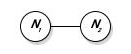
\includegraphics[scale=0.75]{exp1topo.jpg}\newline
Figure 4.1 Experiment 1 Network Topology\end{center}

\noindent It includes three different scenarios to analyze Interest re-transmission between the sender and receiver
nodes. Figure 4.1 illustrates the topology of the network. The following scenarios are tested:

\begin{enumerate}[(a)]
\item No interruptions or disconnections.
\item Link is down from start of run. (Interest not transmitted)
\item Link is down shortly after start of run. (Interest transmitted, response lost)
%% \item Link is down while receiving data. (Interest sent, data interrupted) %% TODO: remove this?
\end{enumerate}

\noindent The following parameters are defined for the scenarios in the experiment:
\begin{itemize}
\item \textsl{Interest timeout period:}  2 seconds
\item \textsl{Interval between Interest re-transmissions:} 5 seconds
\item \textsl{Size of data:} 512 bytes
\end{itemize}

\subsubsection{Scenario 1a: No link disruptions}

This scenario involves no link interruptions or disconnections. It establishes a baseline for delays to be expected under non-impaired network conditions. The receiver (\emph{N\textsubscript{2}})requests information from the sender (\emph{N\textsubscript{1}}). It is expected that the first Interest is immediately satisfied.

\noindent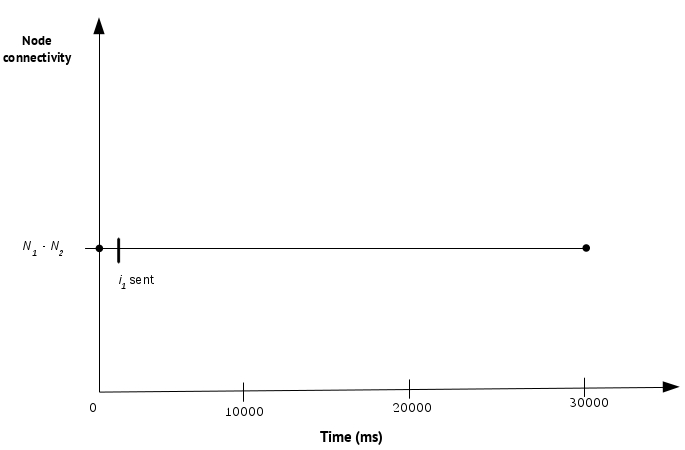
\includegraphics[scale=0.55]{exp1a_timediag.jpg}\newline
\begin{center}Figure 4.2 Experiment (1a) Link between nodes is always up\end{center}

\vspace*{1\baselineskip}\noindent\emph{Observations:}

Based on a number of 10 runs, the experiment runs yield the expected end result of the data being received
based on the first Interest (\emph{i\textsubscript{1}}). The following information shows response times for the requested
data being successfully received:

\begin{center}\textsl{Minimum=522, Maximum=609, Average=538.1 (milliseconds)}\end{center}

\noindent\emph{Discussion:}

As shown in figure 4.2, \emph{N\textsubscript{2}} requests the CCN URI \verb!ccnx://test/1! at the application level which runs on top of the CCNx daemon instance running on the same node. The application sends an Interest 
specifying the URI using the network face that is connected to the daemon. The Interest has a
number of parameters, most notably its lifetime\footnote{The lifetime is not readily configurable based on the implementation code and http://www.ccnx.org/pipermail/ccnx-dev/2010-August/000249.html up to version 0.6.0).}, which is set to 4 seconds for this experiment\cite{CCNxIM}.
The Interest triggers an \verb!interest_from! event on the the local CCNx daemon which results in that
Interest being added to the local \textsl{Pending Interest Table} (PIT) as there is no existing entry. A look-up is then performed on the \textsl{Forwarding Information Base} (FIB) which returns a match for the prefix
\verb!ccnx://test! on a face that connects to the other node. The CCNx daemon then
triggers an \verb!interest_to! event which relays the request over that network face to \emph{N\textsubscript{1}}. Once
the Interest is sent, the CCNx daemon adds the Interest to its PIT.

The CCNx daemon on \emph{N\textsubscript{1}} receives the Interest on its network face and
queries its PIT, which results in no matches. The FIB is then checked for the same prefix and a match is found. The daemon then forwards the Interest to the application face. The application responds by sending back a matching Content Object to the daemon. Signature verification is then performed by the daemon to verify the Content Object integrity. When verification is complete, a \verb!consume! event is issued by the daemon followed by a \verb!content_from! event that identifies that the daemon has sent the data across the network. At this point, the Interest is considered satisfied and can be removed from the PIT.

At this point, the file is cached as a Content Object in the Content Store on  \emph{N\textsubscript{1}}. A
\verb!consume! event followed by a \verb!content_to! event results in the Content Object being sent over the network. The data packet is received on \emph{N\textsubscript{2}}'s daemon and processed through a \verb!content_from! event on the daemon. A look-up is performed in the PIT and a match is found because of the earlier Interest sent by \emph{N\textsubscript{2}}. A \verb!consume! event sends the matching Content Object to the application face interested in the prefix. Finally, a \verb!content_to! event signals that the application reads the data from the local CCN daemon Content Store into memory and writing it to disk to conclude the transfer.

The experiment demonstrates the behaviour of two CCNx nodes in the absence of link disruptions. An average retrieval time of 538.1 ms was recorded.

\subsubsection{Scenario 1b: Link interruption before request is sent}

This scenario tests Interest re-transmission by the receiving node (\emph{N\textsubscript{2}}). This is done by simulating a
loss of connectivity for a duration of 4 seconds when the experiment is first started. It is expected that this loss will result in
the first Interest being sent from \emph{N\textsubscript{2}} to be lost and force a timeout before another Interest is resent, which can then be fulfilled.

\noindent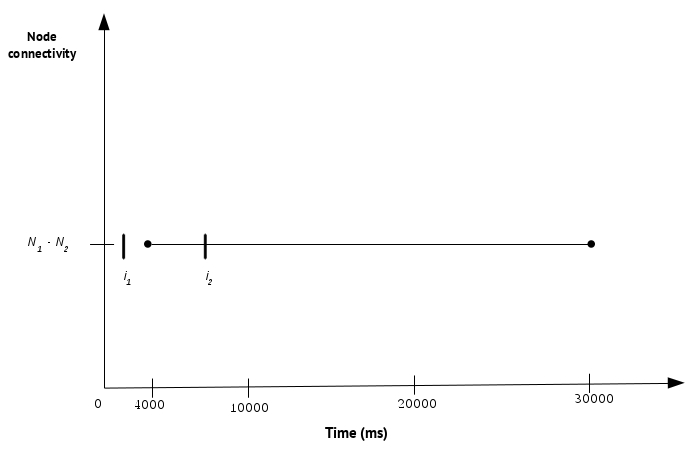
\includegraphics[scale=0.55]{exp1b_timediag.jpg}\newline
\begin{center}Figure 4.3 Experiment (1b) Link down before Interest is sent\end{center}

\vspace*{1\baselineskip}\noindent\emph{Observations:}

Based on a number of 10 runs, the experiments yield the expected end result of the data being received
based on the second Interest. The following information shows response times for the requested
data being successfully received:
\begin{center}\textsl{Minimum=7020, Maximum=7055, Average=7026.3 (milliseconds)}\end{center}

These times are noticeably longer than the ones from experiment 1b. The result recorded is a combination of the timeout period for
the first Interest, the retry interval, and the successful Interest response time.

In addition, the following times identify the response time for the (second) successful Interest:
\begin{center}\textsl{Minimum=19, Maximum=54, Average=25.2 (milliseconds)}\end{center}
These times are much lower than the time recorded in experiment 1a for an immediate (first) successful
Interest.

\vspace*{1\baselineskip}\noindent\emph{Analysis:}

 \emph{N\textsubscript{2}} starts in the same manner it did for experiment 1a as shown in figure 4.3. It requests the CCN URI
\verb!ccnx://test/1! at the application level. A match is not found in the local Content Store or the PIT, so
the Interest is added to PIT for the lifetime of the that Interest. 
The FIB is then searched and a match is found for that prefix. The Interest is sent over the network and
the daemon awaits a response. Because the connection between the two nodes is down at this point in
time, the Interest never reaches  \emph{N\textsubscript{1}}. After a lifetime of 4 seconds, an \verb!interest_expiry!
 event is triggered signalling the end of the lifetime and corresponding entry is removed from the PIT.

The application on \emph{N\textsubscript{2}} is designed to retry the requests 3 times with a retry interval of 4 seconds in
between attempts. After it timeouts from the first Interest, it waits for the user specified retry
interval and sends another request. The second time an Interest is sent, the link between the two
nodes is up and the Interest reaches \emph{N\textsubscript{1}}. On \emph{N\textsubscript{1}}, the CCN daemon receives the Interest and follows the same steps outlined in scenario 1a until the data is received. 

While the total retrieval time is higher to account for the first lost Interest, the response time for the second Interest is lower than in scenario 1a. This is because %% TODO: explain why this is the case!!

\subsubsection{Scenario 1c: Link interruption after request is sent}

This scenario tests Interest re-transmission by the receiving node (\emph{N\textsubscript{2}}). In this case, link interruption is introduced after the Interest is received by the sender node (\emph{N\textsubscript{1}}). It is expected that this interruption will result in the loss of the first Interest and after its lifetime expires, a second Interest is sent, which is then satisfied.

\noindent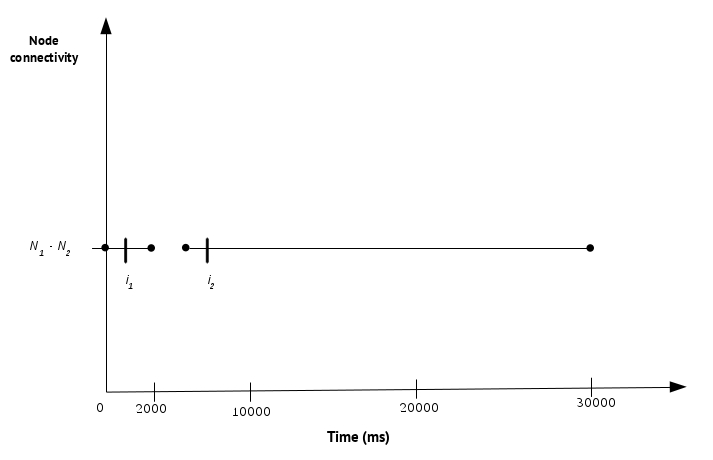
\includegraphics[scale=0.55]{exp1c_timediag.jpg}\newline
\begin{center}Figure 4.4 Experiment (1c) Link down after Interest is sent\end{center}

\vspace*{1\baselineskip}\noindent\emph{Observations:}

Based on a number of 10 runs, the experiments yield the expected end result of the data being received
based on the second Interest. The following information shows response times for the requested
data being successfully received:

\begin{center}\textsl{Minimum=7005, Maximum=7007, Average=7006.33 (milliseconds)}\end{center}

These times are similar to the ones observed in experiment 1b due to the Interest lifetime expiry,
retry delay, and second Interest.

In addition, the following times identify the response time for the (second) successful Interest:

\begin{center}\textsl{Minimum=4, Maximum=6, Average=5.33333 (milliseconds)}\end{center}

These times are much faster than the ones recorded in 1a and 1b.

\vspace*{1\baselineskip}\noindent\emph{Analysis:}

In this scenario, \emph{N\textsubscript{2}} behaves the same way as it did in experiments 1a and 1b. Figure 4.4 illustrates when the Interests
are sent throughout the timeline of the experiment. A request is made for the CCN URI by the application which triggers an Interest that is sent over the network. In this case, the link between the two nodes is up when the Interest is received by \emph{N\textsubscript{1}}, 
however, the link drops before a response in the form of a Content Object is sent back.

\emph{N\textsubscript{1}} follows the normal procedure by searching for the requested prefix in its Content
Store, loading the Content Object from the local application, then sending it back over the network.
However, because the connection is lost by the time the Content Object is sent back, the CCN
daemon on \emph{N\textsubscript{2}} had already expired the Interest from its PIT which results in the Content
Object being discarded. The receiving application will then send a new Interest after its retry
interval elapses, which corresponds to when the connection is restored. This allows the second Interest
to propagate successfully, and the Content Object to be sent back without interruption or delay.

It should be noted that in this case, the Content Object by the CCN daemon on \emph{N\textsubscript{1}}  making
it unnecessary to propagate the Interest to the application running on that node. The prefix is matched
directly to the Content Store and is sent back over the network without intervention from the
application reducing the response time.

%%\subsubsection{Experiment (1d): Link interruption during data transmission}
%% TODO: REMOVE THIS and add in discussion?
%% Insert time action diagram here?
%% \begin{center}Figure 3.x Interest transmission over the duration of the experiment\end{center}

\subsubsection{Conclusion}

Throughout the simple experiments conducted with a single link connecting 2 nodes, it can be
concluded that the CCN daemon does not submit Interest messages other than those expressed by the
application driving the requests. When Interests are lost or not satisfied due to transmission errors, it is
the responsibility of the application to send another Interest until valid data is received. It is
important to note that although the CCN daemon does not attempt to re-transmit Interests itself, it does
provide the capability of validating data being received by matching it to the Interest information as
well as originating Content Object.

In a Delay Tolerant environment, it will be the responsibility of the application to make sure that there
is a continuous stream of Interests to recover from a loss of connectivity.

\subsection{Experiment 2: Network with three nodes and two links}

This experiment involves three nodes, \emph{N\textsubscript{1}} and \emph{N\textsubscript{2}} as well as \emph{R}, which acts as a relay node. \emph{N\textsubscript{1}} is the sender node, while \emph{N\textsubscript{2}} is the receiver following the notation in experiment 1.

\begin{center}
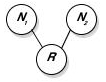
\includegraphics[scale=0.75]{exp2topo.jpg}\newline
Figure 4.5 Experiment 2 Network Topology 
\end{center}

\noindent The experiment tests scenarios similar to the ones outlined in Experiment 1 with the addition of the relay node. Figure 4.5 illustrates the topology of the network. The three scenarios are:
\begin{enumerate}[(a)]
\item Both links are up.
\item Link between \emph{N\textsubscript{1}} and \emph{R} is down before Interest reaches \emph{R}.
\item Link between \emph{N\textsubscript{2}} and \emph{R} is down just after Interest reaches \emph{R}.
\end{enumerate}

\noindent The following parameters are defined for the scenarios in the experiment:
\begin{itemize}
\item \textsl{Interest timeout period:}  2 seconds
\item \textsl{Interval between Interest retries:} 5 seconds
\item \textsl{Size of data:} 512 bytes
\end{itemize}

\subsubsection{Scenario 2a: No link disruptions}

This scenario involves no link interruptions or disconnections. The receiver (\emph{N\textsubscript{2}}) requests information from
the sender (\emph{N\textsubscript{1}}). It is expected that the response data is promptly returned through the relay node. Figure 4.6 illustrates the connectivity between the nodes throughout the timeline of the experiment as well as when the Interest is sent. In this scenario, there is a single Interest that is sent from \emph{N\textsubscript{2}} to \emph{R}.

\noindent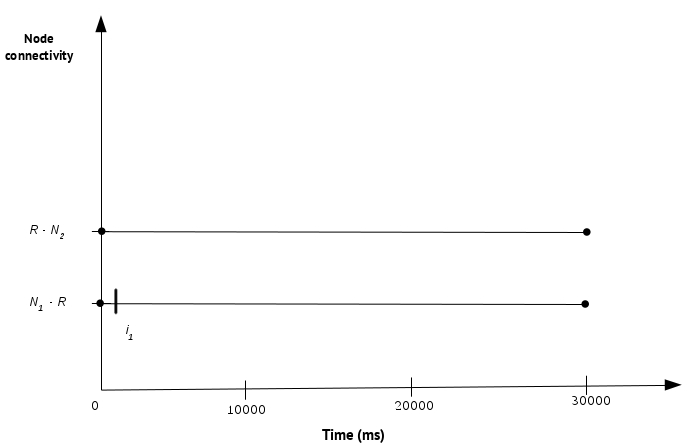
\includegraphics[scale=0.55]{exp2a_timediag.jpg}\newline
\begin{center}Figure 4.6 Experiment (2a) Links between nodes are always up\end{center}

\vspace*{1\baselineskip}\noindent\emph{Observations:}

Based on a number of 10 runs, the experiments yield the expected end result of the data being received
based on the first Interest. The following information shows response times for the requested
data to be successfully received by (\emph{N\textsubscript{2}}):

\begin{center}\textsl{Minimum=32, Maximum=532, Average=176.3 (milliseconds)}\end{center}

In this case,  \emph{N\textsubscript{2}} sends an Interest which must be propagated to  \emph{N\textsubscript{1}}. As an intermediate relay
node,  \emph{R} relays the Interest to  \emph{N\textsubscript{1}}. \emph{N\textsubscript{1}} then sends data back to  \emph{R}, which relays it back to  \emph{N\textsubscript{2}}.

\vspace*{1\baselineskip}\noindent\emph{Analysis:}

The application running on  \emph{N\textsubscript{2}} requests the CCN URI \verb!ccnx://test/1!. The request in the form
of an Interest message is sent to the local daemon instance running on the same node. The Interest is
then added to the local PIT. A look-up is then performed on the FIB which returns a match for
 the prefix \verb!ccnx://test! on a face that connects to \emph{R}. 
When the Interest message reaches \emph{R}, it is added to the PIT. 
The FIB is then searched for the prefix which returns a face connected to \emph{N\textsubscript{1}}. As a result, the
Interest message is then forwarded to \emph{N\textsubscript{1}} where it is also added to the PIT. The prefix matches data
which is locally served by the node, which is consequently retrieved from the application and sent back
over the network. The data first arrives at \emph{R} where it is cached in its Content Store.
The PIT entry for that Interest is removed as it has been satisfied and the data is relayed back to  \emph{N\textsubscript{2}}.

This process is very similar to experiment 1a when there are no disconnections or interruptions
between two nodes. The only exception is the additional relaying operation that is performed by \emph{R}. %%TODO: This needs an explanation as well .. no idea why some are in 250 multiples when the rest are sub 100ms

\subsubsection{Scenario 2b: Link disruption before request is sent}

This scenario involves testing Interest re-transmission by the receiving node (\emph{N\textsubscript{2}}). The link
between \emph{R} and \emph{N\textsubscript{1}} is down at the beginning of the experiment. This link is restored after
four seconds. It is expected that more than one Interest will be sent before the request is satisfied.

\noindent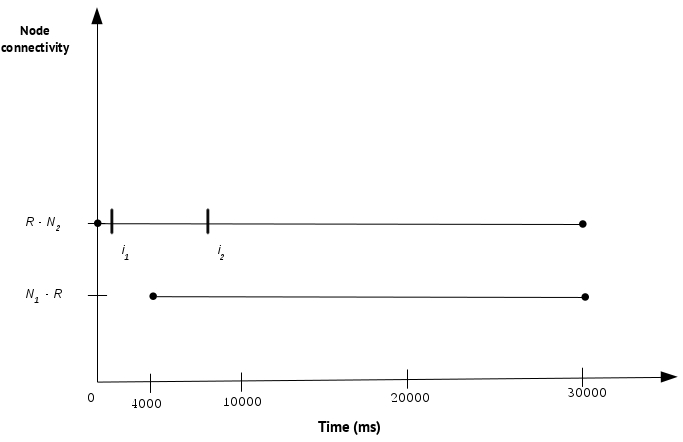
\includegraphics[scale=0.55]{exp2b_timediag.jpg}\newline
\begin{center}Figure 4.7 Experiment (2b) Link between \emph{N\textsubscript{1}} and \emph{R} is down before Interest reaches \emph{R}\end{center}

\vspace*{1\baselineskip}\noindent\emph{Observations:}

Based on a number of 10 runs, the experiments show that two interests are required to successfully
complete the request. The following information shows the total time for the requested data to be
successfully received by  \emph{N\textsubscript{2}}:

\begin{center}\textsl{Minimum=7026, Maximum=7105, Average=7036.9 (milliseconds)}\end{center}

In addition, the following measurements identify the response time for the (second) successful Interest:

\begin{center}\textsl{Minimum=25, Maximum=104, Average=35.9 (milliseconds)}\end{center}

The total time it takes for Interest to be fulfilled is much longer than experiment 2a. This is similar to what was observed in experiment 1b.

\vspace*{1\baselineskip}\noindent\emph{Analysis:}

This is similar to the scenario described in experiment 2a with the exception of the connection between 
 \emph{R} and \emph{N\textsubscript{1}} being unavailable at the start of the run. As shown in figure 4.7, the Interest sent from the application
on \emph{N\textsubscript{2}} reaches \emph{R}, but cannot be relayed to \emph{N\textsubscript{1}} because the link is down. After
the lifetime of the Interest expires, the PIT entries expire on both nodes and the Interest message is
discarded. No Interests reach \emph{N\textsubscript{1}} up to this point.

After the Interest retry interval (5 seconds) elapses, the application on \emph{N\textsubscript{2}} re-sends the Interest
which is then sent to \emph{R} and this time relayed to \emph{N\textsubscript{1}}. \emph{N\textsubscript{1}} 
identifies the URI in the request and replies with the requested data. The data is first cached in the 
Content Store on \emph{R}, then once it arrives at \emph{N\textsubscript{2}} is also cached and forwarded back to the application.

The total time required to fulfill the request is noticeably longer than experiment 2a due to the need for
the second Interest message to be sent. This involves the time required for the Interest message to
expire, the application wait time, the time for the second Interest to be sent, and finally the time it takes
the data to be relayed back.

The time for the successful Interest to be fulfilled is similar to experiment 2a which is expected as after
the first Interest message expires, the entire process must be repeated without knowledge of the prior
attempt. %% TODO: Explain why this is faster

\subsubsection{Scenario 2c: Link disruption after request is sent}

This scenario also involves testing Interest re-transmission by the receiving node \emph{N\textsubscript{2}}. However, in
this case, the link between \emph{N\textsubscript{2}} and \emph{R} is down immediately after the Interest is sent
from \emph{N\textsubscript{2}}. The link between \emph{N\textsubscript{1}} and \emph{R} is operational throughout the experiment. It is expected that more than one Interest will need to be sent before the request is satisfied. Figure 4.8 shows connectivity between the nodes throughout the timeline of the experiment.

\noindent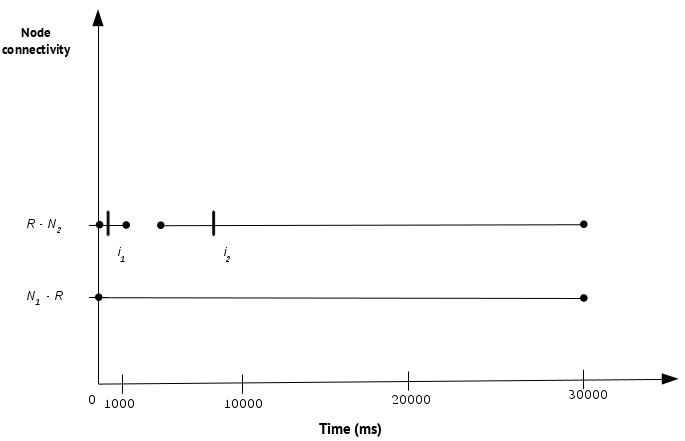
\includegraphics[scale=0.55]{exp2c_timediag.jpg}\newline
\begin{center}Figure 4.8 Link between \emph{N\textsubscript{2}} and \emph{R} is down just after Interest reaches \emph{R}\end{center}

\vspace*{1\baselineskip}\noindent\emph{Observations:}

Based on a number of five runs, the results show that two Interests are required for the request to be
satisfied. The following measurements show the total time for the request data to be successfully
received by \emph{N\textsubscript{2}}:

\begin{center}\textsl{Minimum=7006, Maximum=7008, Average=7007 (milliseconds)}\end{center}

In addition, the following times identify the response time for the (second) successful Interest:

\begin{center}\textsl{Minimum=5, Maximum=7, Average=6.2 (milliseconds)}\end{center}

The times for the successful (second) Interest to be fulfilled are noticeably lower than experiment 2a
and 2b. In addition, while the total time required to fulfill the request is still higher than the one taken
in experiment 2a, it is lower than experiment 2b.

\vspace*{1\baselineskip}\noindent\emph{Analysis:}

This scenario is similar to experiment 2b, except that it forces Interest re-transmission at a different
point of time in the experiment. As opposed to \emph{N\textsubscript{1}} not receiving the first Interest message
in experiment 2b, the first Interest reaches \emph{N\textsubscript{1}} through \emph{R}. However, immediately after the
Interest leaves \emph{N\textsubscript{2}}, the connection between \emph{N\textsubscript{2}} and \emph{R} is lost.

Because the Interest reaches \emph{R}, it is added to its PIT and based on the FIB forwarded to \emph{N\textsubscript{1}}.
\emph{N\textsubscript{1}} then sends the data back to \emph{R}, which attempts to send the data back to \emph{N\textsubscript{2}} but
fails due to the link being down. The PIT entry expires on all 3 nodes, but the Content Object
remains cached in the Content Store of both \emph{R} and \emph{N\textsubscript{1}}.

After the Interest retry interval (5 seconds) elapses, \emph{N\textsubscript{2}} will send another Interest. When this
message reaches \emph{R}, the URI is looked up in the Content Store. Since the corresponding Content
Object is still cached, a response is directly sent back to \emph{N\textsubscript{2}}. \emph{N\textsubscript{1}} plays no
 role in satisfying the second Interest message.

The total time to satisfy the request is slightly shorter than experiment 2b due to the fact that the second
Interest does not need to be sent all the way back to \emph{N\textsubscript{1}}. Additionally, the response time for
the second successful Interest message is noticeably shorter as well confirming that data is being
retrieved from the relay node's Content Store rather than being forwarded on the network.

\subsubsection{Conclusion}

Similar to the conclusion from experiment 1, the application is responsible to ensure that Interests are
re-transmitted as required to fulfill requests. The behaviour of the relay node confirms that CCNx does
not interfere with Interest re-transmission. It also highlights the advantages of caching Content Objects
in the local Content Store which would be an important feature in a Delay Tolerant environment.
Additionally, the introduction of a relay node does not hugely impact performance when tested at
similar connection speeds between the nodes.

It is expected that in a network with more relay nodes, the performance would be similar since re-
transmitted Interests would be satisfied by the closest node on the network. In a Delay Tolerant setting,
it would be beneficial to have Interests re-transmitted at shorter Intervals without explicit requests from
the application. This would ensure that there is a larger window of opportunity around link outages for
the data to be retrieved as well as a greater chance of requested data being cached on more nodes in the
network resulting in faster overall retrieval times.


\pagebreak
\section{DTNx: Enhanced Re-transmission}

From experiments 1 and 2, it was concluded that it would be beneficial to have re-transmit Interests at
shorter intervals without the knowledge of the application. To test this, a separate application, DTNx,
was added to each relay node. The application listens for Interests on the network and continuously re-transmits them until
a corresponding Content Object is received. This mechanism forces the CCNx daemon on each node to keep Interests alive in the PIT 
and increases the probability of both Interest messages and Content Objects being transferred over the network independently of the application sending the original Interest. This allows for data retrieval without end-to-end connectivity between the sender and receiver at any one point in time. It also forces nodes to cache Content Objects along the path the Interests  are sent. DTNx does not manipulate or consume the response data.

To test the effect of DTNx, two additional experiments were performed. Experiment 3 compares the
impact on communication between two nodes, while experiment 4 incorporates three nodes. Each
experiment includes two scenarios which are identical except for the inclusion of DTNx in the second.
In both experiments, three Interests are sent by the application, once per minute. The status of links
between the nodes changes throughout the timeline of the experiment. In scenarios where DTNx is
introduced, it will re-transmit all unsatisfied Interests every five seconds. Re-transmission of a particular
Interest stops when the corresponding Content Object is received. A timeout value of 
three minutes is chosen\footnote{A three minute timeout was chosen as it exceeds the time frame of the experiment.} to avoid endless re-transmission. In a real-life application, the Interest re-transmission interval and the re-transmission timeout value would be dependent on network properties such as connectivity patterns and the cost Interest transmission.

%% Do we really need to mention the next paragraph?
One implementation note that should be mentioned is that due to the inability to control the Interest lifetime
 in the current CCNx implementation, each Interest expression is cancelled three seconds after it is sent on
 both the application and DTNx in order to avoid further automated re-transmission from the CCNx daemon and
 ensure that only one Interest is sent at a time. This workaround has no effect on results as it is consistent 
throughout all experiments.

Observations for experiments 3 and 4 will mainly focus on the effects of DTNx rather than delve into
re-transmission details already described for experiments 1 and 2.

\subsection{Experiment 3: Network with two nodes and one link}

This experiment is similar to experiment 1 with the additional introduction of the DTNx application. The objective is to study the effect of DTNx on Interest re-transmission and performance of the 2-node network. The experiment is split into two scenarios that are based on the same Haggle testbed trace file that specifies when link disruptions will occur. The first scenario uses an unmodified CCNx environment. The second scenario introduces DTNx to the nodes. \emph{N\textsubscript{2}} is the receiving node requesting information and \emph{N\textsubscript{1}} is the sender publishing data. The prime symbol (\emph{\textsuperscript{'}}) indicates that DTNx is running on the node. Figure 4.9 illustrates the topology of the network for Experiment 3.

\begin{center}
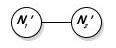
\includegraphics[scale=0.75]{exp3topo.jpg}\newline
Figure 4.9 Experiment 3 Network Topology 
\end{center}

\noindent The parameters used for this experiment are:
\begin{itemize}
\item \textsl{Interest timeout period:} 3 seconds
\item \textsl{Application retry interval:} 60 seconds
\item \textsl{DTNx retry interval:} 5 seconds
\item \textsl{Size of data:} 512 bytes
\end{itemize}

\subsubsection{Scenario 3a: Default CCNx behaviour}

This scenario is similar to scenario 1a except for a longer intervals between Interests sent by the application requesting data. The connection between the node is lost directly after an Interest is transmitted by \emph{N\textsubscript{2}}. The connection is re-established towards the end of the experiment timeline. Because there is no direct connectivity between both nodes until the end of the experiment, it is expected that a response will not be received until then. 

\noindent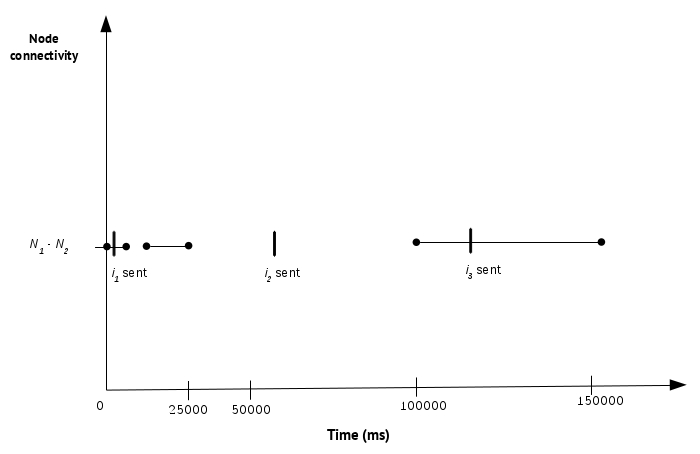
\includegraphics[scale=0.55]{exp3a_timediag.jpg}\newline
\begin{center}Figure 4.10 Re-transmission of Interests generated by \emph{N\textsubscript{2}}\end{center} 

\vspace*{1\baselineskip}\noindent\emph{Observations:}

Based on a number of 10 runs, the results show that 3 Interests are required for the request to be
satisfied. Figure 4.10 maps the Interests sent with the connectivity between the nodes throughout the timeline of the experiment. 
The following measurements show the total time for the request data to be successfully received by \emph{N\textsubscript{2}}:

\begin{center}\textsl{Minimum=126006, Maximum=126036, Average=126014 (milliseconds)}\end{center}

In addition, the following times identify the response time for the (third) successful Interest:

\begin{center}\textsl{Minimum=4, Maximum=34, Average=11.8 (milliseconds)}\end{center}

\vspace*{1\baselineskip}\noindent\emph{Analysis:}

The first Interest from \emph{N\textsubscript{2}} reaches \emph{N\textsubscript{1}} before the link is dropped. The request is fulfilled by the application on \emph{N\textsubscript{1}} and cached in its local Content Store, however, the Content Object is not received by \emph{N\textsubscript{2}}. When the three second request timeout elapses, the application waits for 60 seconds before sending a second request. At that point in time, the link is still down and the Interest is lost. After a further retry interval, a third Interest is sent and the link is up between both nodes. Once received by \emph{N\textsubscript{1}}, the Interest is satisfied directly from the Content Store without intervention from the application. The Content Object is sent back to \emph{N\textsubscript{2}}, where it is cached in the local Content Store and relayed to the application.

\subsubsection{Scenario 3b: CCNx with DTNx on all nodes}

This scenario introduces DTNx on both nodes under the same network conditions as scenario 3a. Because the DTNx application on \emph{N\textsubscript{2}\textsuperscript{'}} re-transmits at a much shorter interval than the application, it is expected that data will be retrieved earlier.

\noindent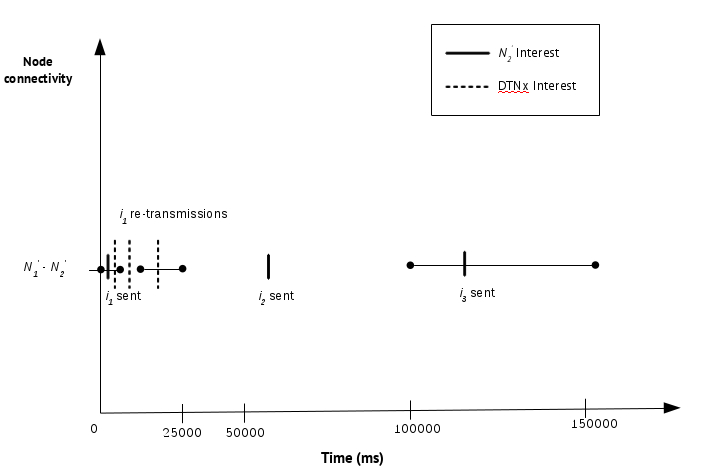
\includegraphics[scale=0.55]{exp3b_timediag.jpg}\newline
\begin{center}Figure 4.11 Re-transmission of Interests generated by \emph{N\textsubscript{2}\textsuperscript{'}} with DTNx\end{center} 

\vspace*{1\baselineskip}\noindent\emph{Observations:}

Based on a number of 10 runs, the results show that two Interests are required for the request to be
satisfied. Figure 4.11 illustrates the points in time when Interests are sent related to node connectivity as well as 
the additional DTNx Interests that are generated. The following measurements show the total time for the request data to be successfully received by \emph{N\textsubscript{2}\textsuperscript{'}}:

\begin{center}\textsl{Minimum=63002, Maximum=63004, Average=63003 (milliseconds)}\end{center}

In addition, the following times identify the response time for the (second) successful Interest:

\begin{center}\textsl{Minimum=1, Maximum=2, Average=1.7 (milliseconds)}\end{center}

The amount of time to receive a response is nearly half the time required for scenario 3a. Additionally, the amount of time for the 
successful interest is also noticeably lower.

\vspace*{1\baselineskip}\noindent\emph{Analysis:}

Similar to the first scenario, the first Interest from \emph{N\textsubscript{2}\textsuperscript{'}} reaches \emph{N\textsubscript{1}\textsuperscript{'}} and is cached locally. Between the first and second Interest sent by \emph{N\textsubscript{2}\textsuperscript{'}}, the DTNx instance on \emph{N\textsubscript{2}\textsuperscript{'}} is continuously sending additional Interests every five seconds. This results in the data being retrieved from \emph{N\textsubscript{1}\textsuperscript{'}} and cached locally on \emph{N\textsubscript{2}\textsuperscript{'}} without the application being aware of it. When the second Interest is sent by the application, it can be retrieved directly from the local Content Store on \emph{N\textsubscript{2}\textsuperscript{'}}. This scenario requires ones less Interest to be sent by \emph{N\textsubscript{2}\textsuperscript{'}} than in experiment 3a because by the time the application sends a second Interest, the data is already locally cached and can be retrieved without relying on the network connection being available.

\subsection{Experiment 4: Network with three nodes and two links}

This experiment is similar to experiment 3 except for the addition for a third node which acts as a CCNx relay node, \emph{N\textsubscript{R}}, between the sender, \emph{N\textsubscript{1}}, and receiver, \emph{N\textsubscript{2}} nodes. The timeline of the experiment is also slightly modified to accommodate the additional link. While scenario 4a tests normal CCNx behaviour, scenario 4b adds DTNx to each of the nodes on the network to gauge its effect. The prime symbol (\emph{\textsuperscript{'}}) indicates that DTNx is running on the node. Both scenarios 4a and 4b use the same Haggle testbed trace file that dictates link disruptions. Figure 4.12 illustrates the network topology for experiment 4.

\begin{center}
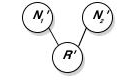
\includegraphics[scale=0.75]{exp4topo.jpg}\newline
Figure 4.12 Experiment 4 Network Topology 
\end{center}

\noindent The parameters used for this experiment are identical to the ones used in experiment 3.

\subsubsection{Scenario 4a: Default CCNx behaviour}

This scenario tests CCNx behaviour in a network with three nodes, one being a relay node. The connection between \emph{N\textsubscript{2}} and \emph{R} is referred to as \emph{Link 1}, while the one between \emph{N\textsubscript{1}} and \emph{R} is referred to as \emph{Link 2}. Figure 4.13 shows the connectivity between nodes throughout the experiment as well as when Interests generated by \emph{N\textsubscript{2}} are sent.

\noindent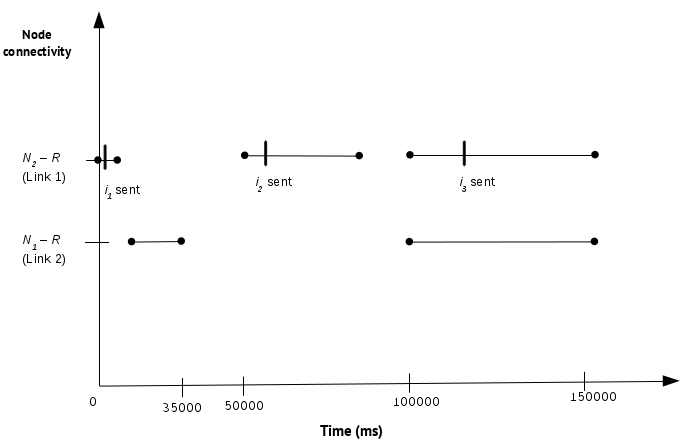
\includegraphics[scale=0.55]{exp4a_timediag.jpg}\newline
\begin{center}Figure 4.13 Re-transmission of Interests generated by \emph{N\textsubscript{2}}\end{center} 

\vspace*{1\baselineskip}\noindent\emph{Observations:}

Based on a number of 10 runs, the results show that three Interests are required for the request to be
satisfied. The following measurements show the total time for the request data to be successfully
received by \emph{N\textsubscript{2}}:

\begin{center}\textsl{Minimum=126015, Maximum=126022, Average=126018 (milliseconds)}\end{center}

In addition, the following times identify the response time for the (third) successful Interest:

\begin{center}\textsl{Minimum=13, Maximum=20, Average=16.6 (milliseconds)}\end{center}

\vspace*{1\baselineskip}\noindent\emph{Analysis:}

The first Interest is sent from \emph{N\textsubscript{2}} to \emph{R}. Because \emph{Link 2} is down, the Interest does not propagate
to \emph{N\textsubscript{1}}. When the second Interest is sent, \emph{Link 1} is again up, but \emph{Link 2} is down, which means this Interest can reaches \emph{R}, but not \emph{N\textsubscript{1}}. When the third Interest is sent by \emph{N\textsubscript{2}}, both links are up and the data can be retrieved successfully through \emph{R}. In this case, the data is only cached locally on each node after the third request is sent. In this scenario, there is a basic end-to-end connectivity requirement between the nodes for the data to be retrieved.

\subsubsection{Scenario 4b: CCNx with DTNx on all nodes}

This scenario is identical to scenario 4a except for the fact that DTNx is running on all nodes. The connection between \emph{N\textsubscript{2}\textsuperscript{'}} and \emph{R\textsuperscript{'}} is referred to as \emph{Link 1}, while the one between \emph{N\textsubscript{1}\textsuperscript{'}} and \emph{R\textsuperscript{'}} is referred to as \emph{Link 2}. Figure 4.14 shows the connectivity between the nodes throughout the experiment as well as the instances where Interests are sent.

\noindent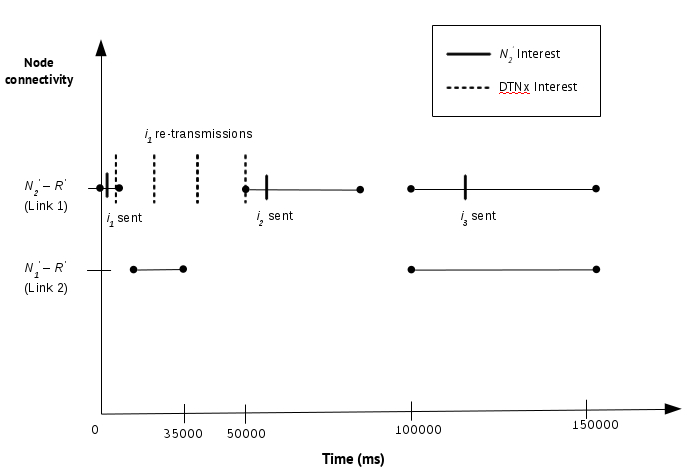
\includegraphics[scale=0.55]{exp4b_timediag.jpg}\newline
\begin{center}Figure 4.14 Re-transmission of Interests generated by \emph{N\textsubscript{2}\textsuperscript{'}} with DTNx\end{center} 

\vspace*{1\baselineskip}\noindent\emph{Observations:}

Based on a number of 10 runs, the results show that two Interests are required for the request to be
satisfied. The following measurements show the total time for the request data to be successfully
received by \emph{N\textsubscript{2}\textsuperscript{'}}:

\begin{center}\textsl{Minimum=63002, Maximum=63003, Average=63002.4 (milliseconds)}\end{center}

In addition, the following times identify the response time for the (second) successful Interest:

\begin{center}\textsl{Minimum=1, Maximum=2, Average=1.6 (milliseconds)}\end{center}

Mirroring the results in experiment 3, scenario 4b shows a noticeably quicker response time for the data as well as the satisfaction time for the successful Interest.

\vspace*{1\baselineskip}\noindent\emph{Analysis:}

The first Interest is sent from \emph{N\textsubscript{2}\textsuperscript{'}} and reaches \emph{R\textsuperscript{'}}. Because \emph{Link 2} is down, the Interest does not propagate to \emph{N\textsubscript{1}\textsuperscript{'}}. When the second Interest is sent, \emph{Link 1} is again up, but \emph{Link 2} is down, which means this Interest also reaches \emph{R\textsuperscript{'}}, but not \emph{N\textsubscript{1}\textsuperscript{'}}. When the third Interest is sent by \emph{N\textsubscript{2}\textsuperscript{'}}, both links are up and the data can be retrieved successfully. In this case, the data is only cached locally on each node after the third request is sent.

In this scenario, the data was retrieved with one less Interest than scenario 4a and much faster, since it is cached locally. Despite there being no direct route between \emph{N\textsubscript{2}\textsuperscript{'}} and \emph{N\textsubscript{1}\textsuperscript{'}} when the first 2 Interests are sent by the application, it is still possible to retrieve the data through \emph{R\textsuperscript{'}} because the increase in frequency of DTNx re-transmission requests results in a higher probability for the window in which a link between 2 of the nodes is up can be taken advantage of.

\subsection{Conclusion}

Experiments 3 and 4 tested the effects of running DTNx on all nodes and the results show that it has proved beneficial. DTNx builds upon fundamental CCN architecture principles to achieve two main goals. Firstly, by re-transmitting more Interests at shorter intervals, more windows of opportunity for end-to-end communication between nodes are created. Secondly, the increase in re-transmission allows nodes to cache Content Objects which in turn enables data retrieval without end-to-end connectivity. In some instances, applications were able to retrieve data from local cache even though the nodes were completely isolated from the network. In scenarios 3b and 4b, there was one less Interest required to retrieve the data compared to scenarios that did not utilize DTNx. 

Although the experiments present a simplified view of connectivity in a controlled environment, they provide valuable insight into factors that have an impact on the introduction of DTNx to the nodes. The number of relay nodes and the re-transmission rate are key variables that could be further investigated to find optimal values best suited for a particular environment. Further experimentation is necessary to identify how those variables would impact larger scale networks. Finally, we believe it would be beneficial to implement re-transmission control mechanisms within the CCNx implementations itself to observe how much of an impact it would have without the overhead of the DTNx layer.

\pagebreak
\chapter{A real application: Delay/Disruption Tolerant Game Platform (DTGP)}

To complement the basic simulations run that test CCNx behaviour in a Challenged Network setting, an
implementation of Tic-Tac-Toe was developed to evaluate its behaviour and performance in a real
application. Tic-Tac-Toe is a two player turn-based game in which players place a mark (normally either X or O)
 on a 3x3 grid in an attempt to complete three of the same mark symbol in a row. 
The main requirements for designing such a game was that it must conform with the
CCNx Interest-driven model and satisfy both conditions of location independence and disruption
tolerance. A framework, referred to as DTGP, was developed to take advantage of CCNx characteristics, 
particularly in relation to delay and disruption tolerance.

In section 5.1, the design of the DTGP framework is introduced with an in-depth discussion of bootstrapping,
addressing, and game state handling. Section 5.2 introduces a number of alternative designs for various aspects 
of the framework with justification as to why they were not chosen. 

Chapter 6 describes experimentation conducted to evaluate the framework by running the Tic-Tac-Toe implementation on the Haggle testbed. Interest re-transmission behaviour and efficiency is determined by analyzing the number of Interests required per game and the Interest satisfaction ratio. The performance is also studied by measuring the satisfaction time for each Interest traversing the network.    

\section{Framework Design}

To implement a CCNx version of Tic-Tac-Toe, we developed a framework to utilize CCNx and potentially be adapted 
for other similar turn-based games. The framework, named DTGP, relies on two main generalization APIs.
Firstly, the network API which is designed around two basic operations: \verb!get! and \verb!put!. These simple
operations abstract the underlying network architecture while maintaining the basic principles of an
ICN. Secondly, the application API which abstracts dependencies between the game and the
network layer to basic functionality such as initialization, running, and terminating. It is up to the game
to implement each of these functions by applying the game logic in conjunction with the network API.

The result is a game that runs on top of CCNx without requiring much understanding from the
developer about the details of an ICN, yet can still function in a Challenged Network setting. It should
also be noted that while the network API used may also theoretically be used with a TCP/IP network,
this has not been tested. An interest message is sent over the network through the \verb!get! method presented
 by the framework, while  a response or Content Object is delivered using the \verb!put! method. 

In the simple scenario of a game of Tic-Tac-Toe, there are two players: A and B which have no prior
knowledge of each other except for being on the CCNx network at some point in space and time. There
are also two distinct types of nodes: 
\begin{enumerate}
\item \emph{Host} nodes that listen for new game requests
\item \emph{Initiator} nodes that send new game requests 
\end{enumerate}

A is a \emph{Host} node that starts running the game first. A initializes a new game object and continuously
 listens for Interest messages from nodes interested in playing a new game. Player B, an \emph{Initiator} node, 
then runs the game and sends Interest messages that request a new game with a unique game ID. The uniqueness of the game ID is
crucial due to the nature of the CCN. This is discussed in some more detail in section 5.1.1. When the
Interests from B reach A, A creates a new game object and sends it back as a Content Object (CO)
to B. When B receives the CO, the Interest for the new game is satisfied and the game can begin.

\begin{center}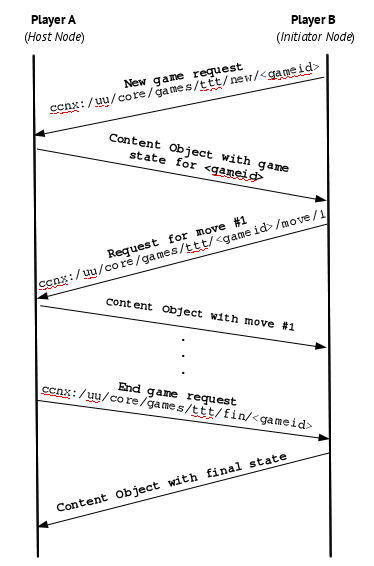
\includegraphics[scale=0.85]{dtgp_msgx.jpg}\newline
Figure 5.1 Illustration of message exchange in a typical game of Tic-Tac-Toe
\end{center}

For simplicity, we assume that \emph{Host} nodes always play the first move. Figure 5.1 illustrates
the message exchange between two nodes in a typical game of Tic-Tac-Toe. After B receives the game CO, a
new request is sent for move \#1. Player A receives the Interest message and sends the response back
followed by a new Interest for move \#2. Player B receives the CO, updates its game state accordingly,
and selects move \#2. Once B receives the request for move \#2 from A, it sends back the updated CO following by an 
Interest for move \#3. The nodes continue to alternate the use of \verb!get! and \verb!put! methods for moves until
 the game reaches a final state at which the winning node will send a finalize Interest message to signal
 that the game has been completed. The response to this request is the final state of the game.

A number of aspects of the design relevant to the principles of the underlying architecture are visited below in more detail.

\subsection{Bootstrapping: Discovery and Initialization}

As is the case with any decentralized design, bootstrapping is always a challenge. In this case, the
characteristics of the underlying ICN architecture are taken advantage of and an opportunistic approach
is followed for nodes to locate others. Following the CCNx protocol, Interest messages are used as a
request mechanism when a node wants to join or start a new game. \emph{Initiator} nodes send out requests in
the form of \texttt{\seqsplit{ccnx://uu/core/games/ttt/new/<gameid>}}, where \texttt{<gameid>} represents a 
unique pseudo-random number. The \emph{Initiator} nodes have no control over which \emph{Host} nodes they are 
matched with as this is purely ad-hoc, based on a first-come-first-serve basis. The uniqueness of the \texttt{<gameid>}
 important to avoid potential conflicts between other games on the network. Nodes active on the network that want to
 play Tic-Tac-Toe passively listen for Interests with a prefix of \texttt{\seqsplit{ccnx://uu/core/games/ttt/new}}. These nodes are referred to as \emph{Host} nodes. The <gameid> portion of the URI is parsed and used to label and a new game instance, which is
then sent back to the \emph{Initiator} node. While it is theoretically possible allow 
all nodes to perform both \emph{Initiator} and \emph{Host} roles, this was restricted to a single role per node for
the purpose of this experimentation.

This initialization process guarantees that opponents will eventually be located because all \emph{Initiator}
nodes are actively advertising their requests and that the underlying architecture provides assurances
that these requests get routed through reachable intermediate CCNx nodes despite there not necessarily
being a direct path to active \emph{Host} nodes on the network.

\subsection{Addressing and Routing}

The framework specifies CCNx URIs based on a name hierarchy that follows the prefix:    
\verb!ccnx://uu/core/games/ttt/!. This assumption simplifies the routing and forwarding mechanism as that is not the focus of this work. That prefix is added to the FIB on each CCNx node so that Tic-Tac-Toe related Interests are propagated throughout to reachable nodes.

Despite the use of this addressing scheme, nodes on the network have no prior knowledge of other
nodes and communication is not end-to-end. Only content is requested and sent back
as a response using the basic Interest and Data messages. Those messages do not specify senders or
recipients, yet are forwarded based on demand. This may result in the network being flooded with
requests before it is fulfilled, however, such a side effect is minimized due to the way the intermediate
nodes do not send out multiple instances of the same Interest that already exists in their PIT. This is
particularly true for situation where there may be more \emph{Initiator} nodes than \emph{Host} nodes resulting in
endless re-transmission of Interests for new games that never get satisfied.

As demonstrated in Chapter 4, interval and timers that control re-transmission can be configured as
appropriate for the state of the network. Although not required for the chosen design, these timers may
also be exploited to expire content on the network sooner than required to avoid Interest message
duplication and conflicts.

\subsection{Game Logic and State}

The framework is designed to support a variety of games, however, given the nature of the underlying
ICN, turn-based games are well suited to demonstrate how tolerant the implementation is
to network delays or disruptions. This is because they have no time constraint requirements and easily fit the
\verb!get! and \verb!put! mechanism presented by the framework. The game logic that runs on the platform will vary
 from one game to another, but still relies on basic \verb!put! and \verb!get! methods presented by the API.

The Tic-Tac-Toe implementation is based on a standard 3x3 grid version. Each player is prompted for
their move on a turn basis. Each time an Interest is received in the form of
\texttt{\seqsplit{ccnx://uu/core/games/ttt/<gameid>/move/<moveid>}}, a Content Object is sent back with the game state
encoded along with the new move requested. There is local input validation for a players move, but
also validation on the remote node. If player A sends back a new game state with an invalid move \#2,
then player B will reject that state and resend a request for the same move while incrementing the id to move \#3. 
Despite the case that player A will make the assumption that the move is valid and proceed to request the next move, 
this request is ignored. Because the players take alternating turns making moves, until player B is satisfied with the new game state, a
request for a new move from player A will not be fulfilled. Player B will keep requesting moves until a
valid game state is returned.

When the game state is evaluated to be final, a \emph{fin} Interest is sent which results in the game ending for
both players. A byproduct of this is that the \emph{new} and \emph{fin} requests can be used as markers for a game to
retrieve and possibly replay it after it has ended. Apart from being useful for analysis, this may also be
used by observers who are able to retrieve the cached copy of the game on the network on a move-by-move basis.

\section{Design alternatives}

There are a number of other designs that were considered, but not implemented or tested. These are
provided below for reference as they try to take advantage of the CCNx protocol differently. These
alternatives are presented but were not part of the experimentation as they either do not strictly adhere
to the CCNx principles of using Interest messages for requesting information and Content Objects for
supplying responses or introduced complexity that made it difficult impractical for experimentation
purposes.

\subsection{Discovery through a centralized directory}

As an alternative mechanism for discovery, another proposed mechanism uses an intermediate node to
act as a “game directory” that acts as a repository for all available games listed by participants on the
network. This approach is suited for situations when routing is based on topological names. While it is
presented as a viable design, it should be noted that it would be unrealistic in a Challenged Network setting
where topology is difficult to predict. 

Player A wants to let the world know that they are available to play a game. The player creates a
Content Object, called a game content object, under the name \texttt{\seqsplit{ccnx://uu/core/games/ttt/open-games/<random-game-id>}}. This Content Object contains the name under which player A wants to receive interests related to the game. For example,\newline

\noindent\textbf{ContentObject URI:} \texttt{\seqsplit{/uu/core/games/ttt/open-games/349057804}}\newline
\textbf{Content:} \texttt{\seqsplit{Player prefix=/vodafone/de/user1/ttt/349057804}}\newline

Player A listens for interests for \texttt{\seqsplit{ccnx://uu/core/games/ttt/open-games/349057804}}, and for interests to
\texttt{\seqsplit{ccnx://vodafone/de/user1/ttt/349057804}}. In an Internet or large network setting, player A may never
receive interests for the former prefix, because there are no routes that point to player A for
\texttt{\seqsplit{ccnx://uu/core/games/}}. The game directory can be thought of as a
database server of open games. Player A sends a \verb!pull! request to the game directory by sending an
interest such as:
\texttt{\seqsplit{ccnx://uu/core/games/ttt/pull-request/\#/vodafone/de/user1/ttt/349057804/game-co}}

This interest is forwarded to the game directory. The game directory sees that this is a registration
request, and identifies the part after the hash sign. It sends a dummy \verb!ACK! content object back in
response to the interest to signal receipt. The game directory then pulls the game object from
player A by sending an interest: \texttt{\seqsplit{ccnx://vodafone/de/user1/ttt/349057804/game-co}}

Player A receives this interest and sends back the game content object. Note that player A cannot send it
back directly, because the game content object is called \texttt{\seqsplit{ccnx://uu/core/games/ttt/open-games/349057804}}, 
and the request was for a prefix of \texttt{\seqsplit{ccnx://vodafone/de/user1/}}. However, player A can still
send a content object that encapsulates the game content object.

When the game directory receives the content object, it imports it to its own namespace. From then
onward, any node on the Internet can now retrieve the game content object
\texttt{\seqsplit{ccnx://uu/core/games/ttt/open-games/349057804}}.

In a Challenged Network, the original registration request may never be received, because player A may not have
connectivity to the game directory. It is still possible, however, for player A to receive interests directly for the
game content object on the \texttt{\seqsplit{ccnx://uu/core/games/ttt/open-games/349057804}} URI. This can only be
considered a fallback mechanism, because the game directory is the main method for game creation.

\subsubsection{Player Matching and Initialization}

Player B joins the network and wants to play a game of Tic-Tac-Toe. Player B sends an Interest for
\texttt{\seqsplit{ccnx://uu/core/games/ttt/open-games/}} and gets back a game content object. It unpacks that content
object and sends out an interest for the player prefix specified in the game content object. In the above
example, Player B sends out an interest as follows:

\texttt{\seqsplit{ccnx://vodafone/de/user1/ttt/349057804/start/\#/twodegrees/nz/user2/ttt/349057804}}

Player A receives this interest, and sends back either a \verb!NACK! (if it has already started the game with
someone else), or an \verb!ACK!, in which case player A and player B are considered to be active participants
of game 349057804. Note that from the Interest message received, player A learns player B's prefix
which follows the hash sign.

While this approach is more complex, it augments the ad-hoc approach with a solution for situations
where Interest message forwarding in a large network is impractical for each node to route based on
published content as opposed to a well defined hierarchy. Because of the large dependency on a centralized game directory, 
this design is not suitable for a Challenged Network environment that is the focus of this experimentation. 

\subsection{Interests as a notification mechanism}

This alternative design uses Interest messages to communicate the current game state instead of Content Objects. The game state is serialized and communicated as a part of the Interest message URI making each request unique for every move as the game progresses. Each Interest has a corresponding Content Object whose purpose is to acknowledge receiving a move. 

Assume that two players have successfully found one another through a discovery mechanism and
have established a game with player A being the one to make the first move. Player A sends an Interest
to player B when it has decided on its first move using \texttt{\seqsplit{ccnx://playerB/<gameid>/<gamestate>}}.
Player B replies with an ACK-type message to acknowledge receipt of the game state. Afterwards,
player B makes a move, updates the game state and sends out an interest as
\texttt{\seqsplit{ccnx://playerA/<gameid>/<updatedgamestate>}} addressed to player A as a notification of the next move.
Player A replies with an \verb!ACK! for this Interest and the cycle continues until the game reaches a final
state.

In this case, each player is responsible for ensuring that its own move it is received by the opponent. While this makes clever use of the messaging mechanism allowed by CCNx, it does not conform to the basic principle of Interests acting as requests and 
Content Objects carrying responses to such requests. Continuously using Content Objects to encapsulate an \verb!ACK! 
does not make efficient use of the protocol. Additionally, this approach does not take advantage of the caching properties of CCNx as the Content Objects do not store any valuable data.

\subsection{Poll driven communication}

Assume that a discovery mechanism is used for two players to identify one another. Player A acts as a
host for the game and player B makes the first move. Player B sends out an Interest message in the
form of \texttt{\seqsplit{ccnx://playerA/<gameid>/move/<i>/<serialized-move>}}. This message specifies the move only 
as opposed to the entire game state. Player A replies with a Content Object that includes the game state
with Player B's move applied to it as well as its own subsequent. When Player B
receives that Content Object, a decision is made based on the new state. Player B's new move is then sent 
in a new Interest message in the form of \texttt{\seqsplit{ccnx://playerA/<gameid>/move/<i+1>/<serialized-move>}}. 
Player A will again apply this move to the game state, decide on a new move, and send a Content
Object back to Player B with the new game state. This continues until the game reaches a final state.

This design is differentiated by the point that one player is entrusted to host the game and maintain the
game state throughout its duration. Each Interest message acts as as both as a request for a new move
and a vessel for the current move. Content Objects carry the updated game state which contains moves
made by the opponent. It is the responsibility of the non-hosting player to ensure that their move is sent
and that a valid game state is received in response.

This approach exploits the messaging mechanism to send data within an Interest and uses Content Objects
as an acknowledgment, albeit carrying the game state. This method again inefficiently utilizes the network and storage space
 as there is duplication of game state data in the Interest and the Content Object. It puts more load on the nodes
to decode each move and apply it to the game state before the logic can be analyzed. It would also make it difficult
for observer nodes to replay the game because requesting a cached move would require knowledge about the move itself.

\pagebreak
\chapter{DTGP Experimentation Using the Haggle Testbed}

A set of experiment runs are used to study the performance of the DTGP framework based on CCNx in a Challenged Network environment.
In all such scenarios, moves for each game are predetermined. This means that each game can be repeated
 while ensuring that it progresses and terminates in the same way for all runs. The \emph{Host} node wins in every run of the experiment. 

\noindent There are two ways to study the data collected from the experiments:

\begin{description}
\item[Application perspective:] This approach focuses on a list of \textsl{unique game messages} composed from
all Interests transmitted by either the \emph{Initiator} nodes or the \emph{Host} nodes. If all interests related to a
game are satisfied, then the game is considered complete.

An Interest is considered satisfied if the original request from an \emph{Initiator} node receives a 
response even though outstanding Interests on relay nodes may not receive a response. The list
of \textsl{unique game messages} is traversed and checked for each \emph{Initiator} node or \emph{Host} node that there
exists a \verb!content_from! message \textit{(inbound response)} for every 
\verb!interest_to! \textit{(outbound request)} message on the same face on the same node.

\item[Network perspective:] This approach focuses on Interests within a game regardless of which node they are
 associated with on the network. Each Interest seen on the network is matched to a
corresponding response.

An interest is considered satisfied if there is a corresponding \verb!content_from! (inbound response) event
for an \verb!interest_to! (outbound request) event on the same face for the same node, regardless of the type
of node. On each node, the list of all messages sent and received are traversed and sorted by timestamp.
Each \verb!interest_to! (outbound request) event is then matched with a \verb!content_from! (inbound response)
response event on the same face. Due to the nature of the experiment, it is common to have a one to
many relationship between \verb!content_from! (inbound response) and \verb!interest_to! (outbound request) events. This is because it is likely that some of the outbound requests are lost. Consequently, the last matched
\verb!interest_to! (outbound request) occurrence from the sorted list is considered to be the actual match for
the response and all other matches are re-transmissions. This is important to both count the number of
re-transmissions for each Interest as well as to calculate the Interest satisfaction time.
\end{description}

\section{Experimentation Parameters} 

Based on a network of five nodes, 21 different experiment runs were executed three times each on the Haggle testbed
using a trace file (see Appendix A) that simulates link disruption over an experiment run duration of one minute. A
combination of \emph{Initiator} and \emph{Host} nodes is varied throughout the different experiment runs, however, there are always
more \emph{Host} nodes than \emph{Initiator} nodes. This is ensure all requests for new games from \emph{Initiator} nodes can be fulfilled
by one or more \emph{Host} nodes. If this ratio is not maintained, there could be a large number of Interests that are never
fulfilled for the entire experiment duration because of insufficient \emph{Host} nodes to fulfill them. 

The haggle testbed trace file used is a one hour truncated version of a ten hour HCMM:SO trace file. It is generated using a simulation of three clusters with five nodes in each that use a Markov model to determine if a link should be up or down at each step in time, depending on the existing state of the link\cite{haggletrc}.
%% TODO might need to fix this paragraph up

\noindent For each experiment run, the CCNd log is analyzed for a number of metrics:

\begin{itemize}
\item \textbf{Interest Satisfaction Ratio:} The ratio is defined as the number of responses for an Interest divided
 by the total number occurrences of that Interest in a run of an experiment.

\item \textbf{Number of Interests per Game:} This metric helps understand the load on the network and the
effects of the disruption on Interest re-transmission by analyzing the number of Interests
required to complete a game. Note that maintaining a high \emph{Host} to \emph{Initiator} node ratio ensures
that all new game requests can be fulfilled successfully based on node connectivity.

\item \textbf{Interest Satisfaction Time:} This metric provides insight into the efficiency of the network in the
face of link disruption by looking at the time it takes to satisfy Interests.
\end{itemize}

\section{Discussion}

In this analysis, the focus is made on the network perspective. This allows us to study the data as a
whole for all nodes and understand the load on the network created by a game as well as how efficiently
requests are forwarded within CCNx on a per Interest level.

Because all games in this experiment reach a final state, there are no unanswered \textsl{unique game messages} that are generated
from the principle nodes of each scenario, whether an \emph{Initiator} node or an active \emph{Host} node. However,
there may potentially be some unanswered requests from relay nodes.

\subsection{Interest Satisfaction Ratio}

The Interest satisfaction ratio provides insight into the amount of overhead required for games to reach a final state in a Challenged Network environment. In the implementation, the total number of responses is divided by the the occurrences for a specific Interest. For example, assume there are 10 occurrences of an Interest, \verb!ccnx://test/1!, and 4 occurrences of a Content Object, \verb!ccnx://test/1/%jhASH@#!. The satisfaction ratio is calculated to be 40\% across the entire network. It should be noted that in the case where there are no responses for a particular Interest, then the satisfaction ratio is calculated to be zero. 

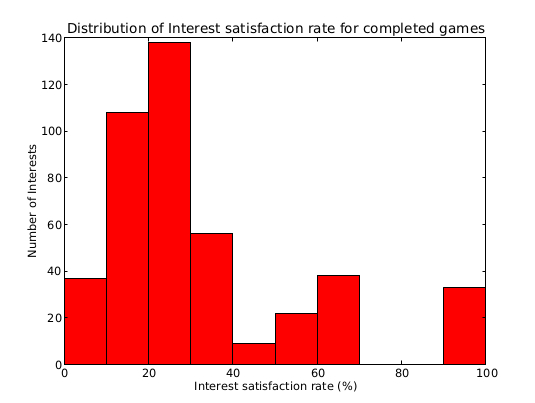
\includegraphics[scale=0.73]{InterestSatisfactionRateHist.jpg}

\begin{center}Figure 6.1 Histogram illustrating the distribution of Interest satisfaction ratio\end{center}

This histogram shows the distribution of the rate at which an interest is satisfied. This is on a per-Interest 
level irrespective of how that Interest may influence a game. It appears that the general case is
that individual interests are rarely satisfied, which correlates to the disruptive nature of the link
configuration in the experiment trace file.

The satisfaction ratio appears to be focused around 20\% for all interests. This means that Interests in some cases may 
need to be re-transmitted five times or more before they are satisfied. While this can be described as a large 
amount of \emph{Interest loss}, this is not to be unexpected considering the nature of the challenged network
 environments being simulated.

\subsection{Number of Interests per Game}

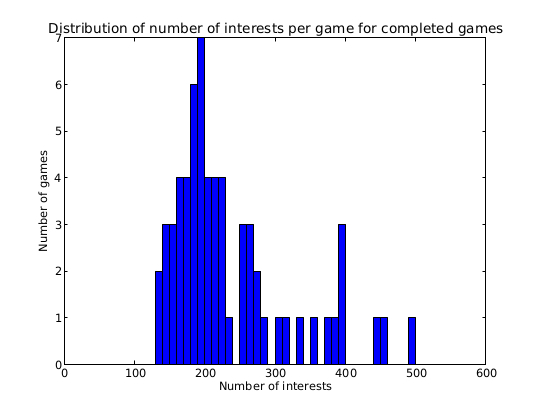
\includegraphics[scale=0.73]{InterestsPerGameHist.jpg}

\begin{center}Figure 6.2 Histogram illustrating the distribution of Interests per game\end{center}

This histogram shows the distribution of the number of Interests required to complete a game. 
Based on this experiment trace, there are no games that do not result in a final state.
The number of Interests required to complete a game for most cases is approximately 200 Interests. 

It is unclear why this is the optimal number of Interests required, but this is likely to be due to a number of factors.
Each game requires a minimum of seven interests to reach a final state by each \emph{Initiator} node. Based on the
20\% satisfaction rate observed and the five nodes participating in the network, the number of Interests is close to
the most prominent rates displayed in figure 6.1. Additionally, while there is no measurable impact, we believe that the link disruptions in the trace file have a large impact on the number of re-transmissions required.  
%% TODO discuss this number discrepancy with Frederik

\subsection{Interest Satisfaction Time}

The Interest satisfaction time is defined by the time it takes for a node on the network to receive a response for an Interest that it
sent. There are three different methods to calculate satisfaction time for an Interest. As discussed earlier,
Interests have no inherent state or sequence identification which makes it difficult to differentiate or
track the interests.\footnote{While it may be possible to use the nonce associated with Interest messages for uniqueness, this is not investigated in this study.} 
Note that an interest can only be identified by the message itself, the node it was seen on, and which face on which it was transmitted.

\begin{enumerate}
\item Use the first occurrence of an Interest on a node as the baseline for response time calculation. This
works under the assumption that one wants to measure how long it took to get a response from the first
request transmitted by a node on the network.
\item Use the last occurrence of an interest on a node as the baseline for response time calculation. This
would work in the case that one assumes that the latest Interest sent by a node is the one that triggered a
response, even though it may have not been the initial trigger. To elaborate, a previous Interest may have cached
 the response on a relay node nearby and this final interest pulled the cached copy.
\item Attempt a rather complex solution which involves tracking a Interest through every single \textsl{hop} and
use the hop aggregates to calculate the response time. This would probably provide the most accurate
response time for the interest that was actually satisfied, however, this approach runs into ambiguity in
terms of which Interest actually triggered the response. If it takes three separate Interest re-transmissions to
get the data cached to an adjacent node on the network and a final fourth Interest to actually pull the
response, it becomes difficult to identify which of those interests would be the baseline to use for the
calculation.
\end{enumerate}

The first approach is chosen as it provides a simple and straight-forward approach to identify the
response time for an Interest on the network. As a result, this metric only deals with unique game
messages on the network rather than treat Interests transmitted on the network on an individual
basis. While this provides an arguably narrower data set, it removes any ambiguity from approach \#3
related to matching Interests and their corresponding responses which cannot be uniquely identified
being a basic principle of a CCN.

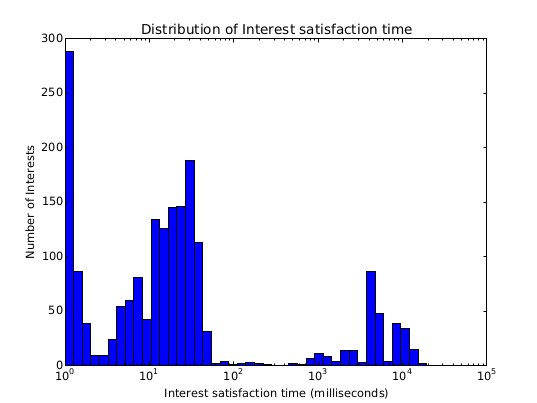
\includegraphics[scale=0.73]{InterestResponseTimeHist.jpg}

\begin{center}Figure 6.3 Histogram illustrating the distribution of individual Interest satisfaction time on a logarithmic scale\end{center}

The histogram shows that the majority of Interests on the network are satisfied within 200 milliseconds
and most just under a few milliseconds. This is likely to be due to the constant caching of responses
throughout the network when a window of opportunity arises for communication between nodes when
the links are up. This highlights efficiency in the network despite the disruptions that regularly take
place.

There are some outliers in the data for which the satisfaction time may be up to 19 seconds. This is
arguably a considerable amount of time when the duration of the experiment is 60 seconds. However, it
should be noted that some of the Interests which have a longer response time may have been ones
triggered by relay nodes which would not necessarily have hindered game progression.

\section{Conclusion}

The outcome of the experimentation meets expectations in terms of Interest re-transmission behaviour and performance.
Despite the number of moves required to reach a final state in optimal conditions are low, there is a high number of Interests observed for for each game.
This correlates to a low Interest satisfaction ratio. Despite this, the Interest satisfaction time is low with each game completing within the experiment timeframe.
This means that while the network might be slightly overloaded due to increased re-transmissions, the requests are promptly satisfied which is a good trade-off in a Challenged Network environment.

\pagebreak
\chapter{Related Work}

The term Information-Centric Networking defines a rather large subset of protocols that share the some
fundamental characteristics. While separating information retrieval from being location dependent is
the fundamental pillar of ICNs, some approach the problem differently. This may influence the
characteristics of the network and how it behaves in certain conditions, such as Challenged Networks.

This section looks at the broader family of Content-Centric Network protocols, of which CCNx is one
implementation, and compares them to how other Information-Centric protocols perform in a
Challenged Network environment. The differences discussed include data distribution mechanisms,
naming and addressing schemes, routing, caching, and tolerance to mobility or disruption\cite{dirk2941}.

\section{Publish-Subscribe Based Models}

The \textbf{Publish-Subscribe Internet Routing Paradigm (PSIRP)} is a publish-subscribe based protocol
that involves source nodes publishing content on the network. Nodes that want to receive the data must
subscribe to specific content. A Rendezvous system matches the publishers with the subscribers and
produce identifiers that form communication channels and forwarding routes that route data between
the nodes.

\textbf{Network of Information (NetInf)} is another publish-subscribe based protocol in which source nodes
publish objects to the network through a Name Resolution Service which also stores an associated list
of network locators for that object. A request can then be sent to the NRS to retrieve the network
locators through which the object can be retrieved.

\textbf{Data-Oriented Network Architecture (DONA)} uses a hierarchical resolution infrastructure to
authorize data that is published by nodes. A registered object is considered valid for a certain period of
time and has a route associated with it to the source node. A request is propagated through the
resolution infrastructure in an attempt to fulfill it through the closest node that has a copy of the data.
Registrations can be using wild cards to force requests to a specific node without specifying one object
a time. Data responses will generally be routed back along the same path the request was received.

%[ mechanism, addressing ]
The aforementioned models differ from CCNs as they depend on a registration or publish-subscribe
mechanisms. They are based on a flat naming scheme used for their addressing mechanism. With the
exception of NetInf which is purely flat, the other models use a hierarchical name resolution system
similar to the Internet's DNS architecture and make use of Bloom filters for improved look-up
performance. The CCN hierarchical prefix aggregation model is inherent in the architecture of the
protocol which offers advantages in terms of routing performance scalability on larger scaled networks.

%[caching]
\emph{In-network caching} is an inherent characteristic shared between the models. The request driven models
follow an opportunistic method for caching data as it is seen on the network, usually as a response to a
data request. Some models such as NetInf have the added ability to cache data through direct requests
to the name resolution system if the requested data is registered with it. PSIRP restricts the caching to
the scope of an object's rendezvous point. CCNs are unique in the sense that it could support a finer granularity of caching based on smaller parts of a data objects that are fulfilled from different nodes on
the network. Space in caches can be freed by deleting objects based on available capacity based on
various factors, such as aging. These caching mechanisms are more effective than edge network
caching as they focus on active data on the network based on demand among a group of nodes as
opposed to needlessly replicating data to all nodes on the network potentially wasting storage and
bandwidth capacity.

%[ mobility/disruption tolerance ] - add these comments as review/markup
Disruption tolerance and mobility are two of the areas that CCNs stand out compared to the other
publish-subscribe models. In a Challenged Network environment where connectivity is sparse, location
transparency with respect to other nodes on the network is a crucial factor. CCNs inherently support
this behaviour through the strategy layer that allows communication over any of the available interfaces
on a node regardless of the connectivity state with the network. On the other hand, the publish-
subscribe models discussed all require some form of registration with a name resolution system or rely
on a common rendezvous service. These protocols suffer greatly in this regard because direct
connectivity can not guaranteed. This is especially true for the relocation of source nodes that must re-
register before their information objects can be retrieved on the network\cite{dirk2941}.

\section{NDN Protocols}

Being a subset of ICNs, NDN based protocols share a lot of common properties with CCNs.
\textbf{BOND} \cite{bond} is a broadcast protocol which is based on named data and is independent of the
level of connectivity or mobility between nodes on the network. This is similar to CCNx in that it
attempts to utilize any available communications link to reach other nodes.

Like CCNx, BOND is also requester initiated. Requests, which are similar to Interests, are sent
for named data on the network which are then forwarded to reachable nodes until the request reaches a
node on the network which holds the data. The response is used to both learn the route back to the
requester as well as cache the data locally on each node along the route to fulfill future requests. Prefix
matching is used to identify which requests can be satisfied or forwarded. Additionally, BOND
maintains data structures to keep track of messages including a Distance Table, Pending Send Index,
and a Cache Store, which are synonymous to the FIB, PIT, and Information Store used by CCNx,
respectively.

When processing request packets, BOND considers 2 main factors on a per node basis: 1) \textit{Can a
node forward the request?} 2) \textit{How long to wait before forwarding the data back to the sender?} The
decision on whether to forward or not is based on a distance metric between the sender and the
requesting node. Nodes that are too far away are ineligible. Eligible nodes compete on whether to send
the data based on a randomly based delay metric to avoid collision. Each packet sent on the network is
identified by a nonce which is used to decide on whether it should respond to that request packet seen
on the network or ignore it. This is similar to strategy and suppression rules that CCNx employs to
control how responses are sent by nodes on the network and avoid response duplication. One difference
with flow control is how BOND nodes will explicitly acknowledge receipt of data packets to avoid
unnecessary data being sent to the requesting node after it's request is satisfied. CCNx avoids this
mechanism and replies on the requesting node to ignore duplicate packets.

BOND classifies connectivity into connected and disconnected networks which affect its mode
of operation. Nodes will react differently if they detect that they are in a disconnected network. When
this mode is enabled, nodes will automatically resend packets using what is named a replay flooding
technique. CCNx once again takes the simpler approach and relies on the requester to ensure data is
successfully retrieved with no guarantees provided by other nodes on the network.

While the BOND design does not mention the use of multiple interfaces in a way that CCNx
does, this functionality may be inherent in the way the broadcast mechanism works. However, BOND
explicitly uses layer 2 MAC transmission with custom collision avoidance mechanisms and cannot run
on top of higher level (TCP/UDP) protocols like CCNx can. While this is theoretically not a
disadvantage, it limits the practical use of the protocol as it cannot be used in hybrid connected and
disconnected networks that run over IP.

Overall, both implementations approach the problem in a very similar fashion and as a result
would be expected to perform as such. The disconnected mode BOND uses will provide assurances
that data delivery will continue in a challenged network environment where there are delays or link
disruptions. It is possible that the more complex BOND approach for data delivery may improve
performance and reduce packet redundancy, however, it is likely that it will not be much of an
improvement over CCNx.

\section{Opportunistic Network Protocols}

Another architecture commonly associated with Challenged Networks is Opportunistic Networking. In
Opportunistic Networks, nodes use their locality to determine the best route throughout the network.
When a message or packet is to be sent across the network, a node will independently determine the
next hop based on the final destination. If such a hop is not immediately available, the forwarding
decision is delayed until a later time. While this architecture does not guarantee speedy delivery, its
flexible nature is well suited for environments where connectivity is unreliable, either due to delays or
disruption\cite{oppnets}.

\pagebreak
\chapter{Conclusion}

This work investigated the effects of using a Content-Centric Network in a Challenged Network environment. CCNx was the chosen
CCN implementation to use along with the Haggle testbed to simulate loss of connectivity between nodes. Experiments were
conducted to study the Interest re-transmission as a result of link disruption in simple network topologies. The
information learned from those experiments were then applied for a more complex analysis that involved running a
game of Tic-Tac-Toe under similar conditions. The analysis helped identify some aspects of the behaviour and performance of
running CCNx in a more practical application.

The results from the experiments in Chapter 4 demonstrated that CCNx can handle link disruptions well. With inherent CCNx re-transmission
disabled to create a controlled environment with two nodes, it is the responsibility of the application requesting information to ensure that messages are received. Due to the nature of the network, there is no way to verify that Interest messages have been received by the other node except for when the corresponding Content Object is received by the same node that sent the Interest. With the introduction of a relay node, the efficiency increases because the intermediate nodes allow for both a better window of opportunity for message transmission as well as an enhancement of the caching mechanism inherent on each node on the network. We believe that the introduction of further relay nodes will further enhance the performance. We also believe that if the re-transmission timers on each node were shortened, it would reduce the amount of time taken for an Interest to be satisfied. In contrast to a TCP/IP, the experiments highlight that no end-to-end connectivity is required for data retrieval. They also proved that the data need not be retrieved for one particular node, which reinforces the advantage of the location transparency in CCNx.

In Chapter 5, Tic-Tac-Toe was implemented on top of a framework that was developed based on CCNx. This allowed for further experimentation in a more complex network with more nodes. The inherent CCNx re-transmission mechanism was unhindered in this experiment. The results show that there is a large amount of Interest re-transmission required to cope with the link disruption on the network. Despite this, the satisfaction time for each Interest is still quite low. The results from Chapter 4 and Chapter 5 lead us to believe that CCNx could be applied in real world applications where such an architecture would be advantageous. In cases where connectivity is intermittent and predictable, such as bus routes, CCNx could excel when re-transmission variables are appropriately configured.

Overall, we believe that content-centric networking is a good contender for use within Challenged Network environments. While much experimentation is still required to fine-tune variables involved, its inherent properties overcome many of the shortcomings of traditional TCP/IP networks. 

\pagebreak
\chapter{Future Work}

Additional experimentation and analysis is necessary to further understand how to enhance the performance of CCNs in Challenged Networks. The following proposals are provided as guidance for future research that can build on this existing work.

\begin{itemize}
\item The optimal number of relay nodes that enhance Interest response time should be investigated. This can be done by gradually increasing the number of nodes in the network and comparing Interest satisfaction times. It should also be noted that having too many nodes may overload the network and thus a balance must be found to make efficient use of the transmission medium.

\item The amount of caching by each of the nodes on the network should be studied. This study would find the most suitable cache size required on each node, keeping in mind that space is likely to be an expensive resource on nodes in this type of network.

\item Further experimentation with internal CCNx re-transmission intervals is necessary to identify whether flooding the network with more requests will result in faster satisfaction times or not. While the tests in Chapter 4 attempt to test this by adding DTNx as an additional application on each node, modifying the interval on the CCNx is likely to present different results.

\item It may be possible to introduce some adaptive (learning) transmission mechanism over time to avoid
overly re-transmitting Interests when we have no connectivity. This may improve the Interest satisfaction ratio considerably. Even though it is unlikely that satisfaction time would decrease dramatically, the amount of outliers should be reduced.

\end{itemize}

\pagebreak
\bibliography{mybib}{}
\bibliographystyle{plain}

\pagebreak
\chapter*{Appendix A: Tic-Tac-Toe Haggle testbed Scenario}

Haggle testbed trace file that specifies duration for link up-time between nodes for 5 nodes and
duration of 1 minute.

\small\begin{verbatim}
---- Start of File ---------
5	1	84	97
1	5	84	97
3	2	71	100
2	3	71	100
5	1	113	114
1	5	113	114
5	2	147	252
2	5	147	252
5	4	243	278
4	5	243	278
3	1	189	319
1	3	189	319
3	1	333	365
1	3	333	365
4	3	380	393
3	4	380	393
5	2	388	395
2	5	388	395
5	3	342	403
3	5	342	403
3	2	336	418
2	3	336	418
4	1	350	436
1	4	350	436
5	4	374	480
4	5	374	480
5	1	522	537
1	5	522	537
5	3	577	579
3	5	577	579
4	3	565	645
3	4	565	645
5	1	615	659
1	5	615	659
3	2	679	684
2	3	679	684
5	4	684	696
4	5	684	696
4	2	720	736
2	4	720	736
3	1	658	750
1	3	658	750
5	3	641	771
3	5	641	771
5	1	718	776
1	5	718	776
3	2	765	777
2	3	765	777
4	2	847	864
2	4	847	864
5	3	841	880
3	5	841	880
5	1	878	884
1	5	878	884
5	4	858	888
4	5	858	888
5	2	841	889
2	5	841	889
4	3	1007	1038
3	4	1007	1038
5	4	1007	1111
4	5	1007	1111
4	3	1140	1141
3	4	1140	1141
3	1	971	1165
1	3	971	1165
5	3	1118	1208
3	5	1118	1208
4	2	1209	1223
2	4	1209	1223
3	2	1150	1243
2	3	1150	1243
4	3	1197	1251
3	4	1197	1251
5	3	1242	1280
3	5	1242	1280
3	2	1269	1307
2	3	1269	1307
3	2	1339	1340
2	3	1339	1340
3	2	1357	1368
2	3	1357	1368
5	1	1230	1375
1	5	1230	1375
5	2	1377	1420
2	5	1377	1420
4	2	1382	1426
2	4	1382	1426
4	3	1449	1513
3	4	1449	1513
5	1	1498	1567
1	5	1498	1567
5	4	1552	1571
4	5	1552	1571
5	3	1560	1573
3	5	1560	1573
5	4	1707	1712
4	5	1707	1712
4	2	1711	1720
2	4	1711	1720
4	3	1628	1743
3	4	1628	1743
4	1	1696	1744
1	4	1696	1744
4	1	1764	1794
1	4	1764	1794
3	1	1783	1795
1	3	1783	1795
5	2	1820	1823
2	5	1820	1823
5	2	1843	1918
2	5	1843	1918
5	3	1903	1930
3	5	1903	1930
4	1	1815	1937
1	4	1815	1937
5	2	1960	1969
2	5	1960	1969
5	3	2018	2030
3	5	2018	2030
5	3	2031	2043
3	5	2031	2043
3	2	1976	2046
2	3	1976	2046
3	2	2058	2075
2	3	2058	2075
4	2	2064	2109
2	4	2064	2109
2	1	2026	2114
1	2	2026	2114
4	2	2119	2168
2	4	2119	2168
4	1	2149	2179
1	4	2149	2179
5	2	2217	2223
2	5	2217	2223
5	3	2218	2275
3	5	2218	2275
3	1	2076	2302
1	3	2076	2302
3	1	2309	2321
1	3	2309	2321
4	3	2319	2363
3	4	2319	2363
3	2	2330	2371
2	3	2330	2371
3	1	2457	2468
1	3	2457	2468
3	2	2379	2486
2	3	2379	2486
5	2	2431	2493
2	5	2431	2493
4	1	2382	2534
1	4	2382	2534
3	1	2522	2580
1	3	2522	2580
4	2	2535	2592
2	4	2535	2592
5	4	2586	2609
4	5	2586	2609
4	3	2615	2618
3	4	2615	2618
4	1	2558	2626
1	4	2558	2626
5	1	2664	2718
1	5	2664	2718
5	2	2548	2727
2	5	2548	2727
4	2	2774	2784
2	4	2774	2784
5	2	2755	2814
2	5	2755	2814
5	4	2845	2852
4	5	2845	2852
5	3	2811	2865
3	5	2811	2865
5	1	2786	2873
1	5	2786	2873
4	3	2878	2894
3	4	2878	2894
4	2	2977	2984
2	4	2977	2984
5	3	2980	2997
3	5	2980	2997
3	2	3004	3006
2	3	3004	3006
4	3	2927	3006
3	4	2927	3006
4	3	3049	3093
3	4	3049	3093
5	2	3033	3100
2	5	3033	3100
5	4	3081	3118
4	5	3081	3118
4	1	3175	3184
1	4	3175	3184
5	4	3139	3194
4	5	3139	3194
3	1	3142	3196
1	3	3142	3196
4	3	3217	3225
3	4	3217	3225
4	2	3226	3227
2	4	3226	3227
4	1	3205	3228
1	4	3205	3228
5	1	3051	3249
1	5	3051	3249
5	4	3208	3262
4	5	3208	3262
4	2	3263	3270
2	4	3263	3270
3	1	3206	3314
1	3	3206	3314
5	1	3276	3325
1	5	3276	3325
5	2	3315	3343
2	5	3315	3343
3	2	3308	3361
2	3	3308	3361
3	1	3349	3380
1	3	3349	3380
4	1	3430	3441
1	4	3430	3441
5	2	3418	3457
2	5	3418	3457
5	3	3430	3516
3	5	3430	3516
4	3	3506	3524
3	4	3506	3524
2	1	3548	3600
1	2	3548	3600
------ End of File ---------

\end{verbatim}

\end{document}               % End of document.

